\chapter{Systemdesign}

Da der Feasibility Check als Funktionalität in die bestehende Software-Applikation \gls{REALIS} integriert werden soll, ist es notwendig, die bereits verwendeten Technologien und Programmiersprachen sowie die Architektur zu übernehmen, um eine nahtlose Integration zu gewährleisten.

Eine Evaluierung alternativer Technologien, die möglicherweise besser für die Applikation geeignet wären, wurde daher nicht durchgeführt. Stattdessen orientiert sich die Umsetzung strikt am bestehenden System.

Für das Datenbankdesign kommt eine Oracle-Datenbank mit SQL zum Einsatz. Die Backend-Logik wird in der objektorientierten Programmiersprache C\# implementiert. Für das Frontend wird das Webapplikationsframework Angular verwendet, das auf TypeScript basiert. Angular ermöglicht eine parallele Entwicklung sowohl für Webanwendungen als auch für native Mobilapplikationen.

\section{Architekturüberblick}

Die Abbildung 4.1 veranschaulicht die erweiterte REALIS-Architektur zur Realisierung des Feasibility Checks. Basierend auf dem bestehenden REALIS-Komponentendiagramm (siehe Abbildung 2.3) werden neue Komponenten hinzugefügt, um die Feasibility-Check-Funktionalität zu integrieren. Im Diagramm sind dabei aus Gründen der Übersichtlichkeit nur die wichtigsten Erweiterungen dargestellt.

\begin{figure}[!htbp]
    \centering
    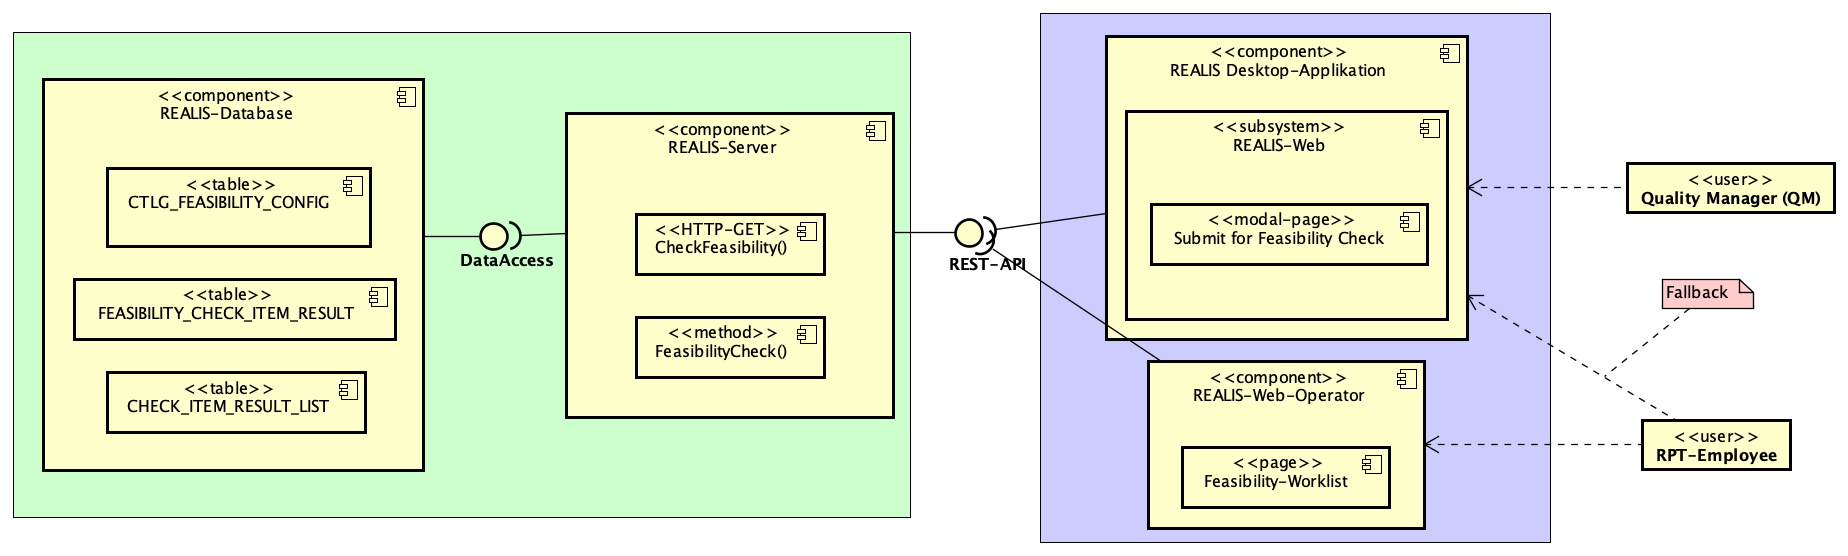
\includegraphics[width=1\textwidth]{bilder/Feasibility-Komponentendiagramm.png}
    \caption{Feasibility Check Architekturdesign-Erweiterung von \gls{REALIS}}
    \label{fig:feasibility-check-komponentendiagramm}
\end{figure}

\todo{maybe add opdataparamtype}

In der \textbf{Datenbank} werden neue Tabellen hinzugefügt, die sowohl zur Konfiguration als auch zur Speicherung der Check-Ergebnisse dienen. Hierzu gehören die Tabellen \texttt{CTLG\_FEASIBILITY\_CONFIG}, \texttt{FEASIBILITY\_CHECK\_ITEM\_RESULT} und \texttt{CHECK\_ITEM\_\-RESULT\_\-LIST}.

Im \textbf{Backend} wird eine HTTP-GET-Methode mit der Bezeichnung \texttt{CheckFeasibility()} implementiert. Diese Methode ruft die Kernlogik der Funktion \texttt{FeasibilityCheck()} auf, die die eigentliche Datenverarbeitung übernimmt, die Ergebnisse in der Datenbank abspeichert und ein einfaches Ergebnis zurückliefert.

Im \textbf{Frontend} werden Erweiterungen in zwei Bereichen vorgenommen: Im \textit{REALIS-Web Subsystem} wird eine neue Modal-Page \glqq Submit for Feasibility Check\grqq{} integriert, die es Benutzern ermöglicht, den Feasibility Check zu initiieren. Zusätzlich wird in der Komponente \textit{REALIS-Web-Operator} eine neue Webpage \glqq Feasibility-Worklist\grqq{} hinzugefügt, welche die Ergebnisse des Feasibility Checks sowie offene Aufgaben übersichtlich darstellt.

Durch diese Erweiterungen wird die Feasibility-Check-Funktion nahtlos in die bestehende REALIS-Architektur eingebettet und ermöglicht eine effiziente Interaktion mit den relevanten Benutzern und Systemkomponenten.




\section{Datenbankdesign}
Um die Erweiterung der Datenbank für den Feasibility Check zu erklären, wird zunächst auf die grundlegende Struktur der REALIS-Datenbank eingegangen. In Abbildung \ref{fig:realis-datenbankdesign} ist ein Ausschnitt der wichtigsten Tabellen und deren Beziehungen zueinander dargestellt, einschließlich der vorgenommenen Erweiterungen, die durch orange Rechtecke gekennzeichnet sind. In den folgenden Erläuterungen sind die zugehörigen Tabellennamen aus der Abbildung \ref{fig:realis-datenbankdesign} jeweils in Klammern angegeben.

\subsection{REALIS-Datenbank}

Wie bereits in Kapitel \ref{Subsec:project-lifecycle} beschrieben, besteht ein \textbf{REALIS-Projekt} (\texttt{relproject}), das zur Qualifizierung neuer Produkte dient, aus mehreren \textbf{Tests} (\texttt{test}). Jeder Test besitzt einen eindeutigen \textbf{Status} (\texttt{ctlg\_state\_type}), der zu Beginn auf ''NEW'' gesetzt wird und nach Abschluss den Status ''ARCHIVE'' erhält (vgl. Abbildung \ref{fig:realis-project-lifecycle}, rechte Spalte). Zudem wird jeder Test einer Kategorie bzw. einem \textbf{Test-Typen} (\texttt{ctlg\_\-test\-\_sub\_type}) zugeordnet.

Ein Test besteht aus mehreren aufeinanderfolgenden \textbf{Operationen} (\texttt{operation}), die nacheinander im \gls{RPT}-Labor abgearbeitet werden. Die Tabellen, die eng mit der Operation verknüpft sind, sind in Abbildung \ref{fig:realis-datenbankdesign} im grün umrandeten Bereich dargestellt. Jede Operation kann dabei einen oder mehrere \textbf{Parameter} (\texttt{op\_data}) enthalten, die beispielsweise die Umgebungsbedingungen definieren. Die konkreten Werte dieser Parameter sind in dem Eintrag \texttt{OPD\_PLAN} hinterlegt. Jedem Parameter wird außerdem ein \textbf{Parameter-Typ} (\texttt{ctlg\_op\_\-data\_type}) zugewiesen.  


\begin{figure}[!htbp]
    \centering
    \makebox[\textwidth]{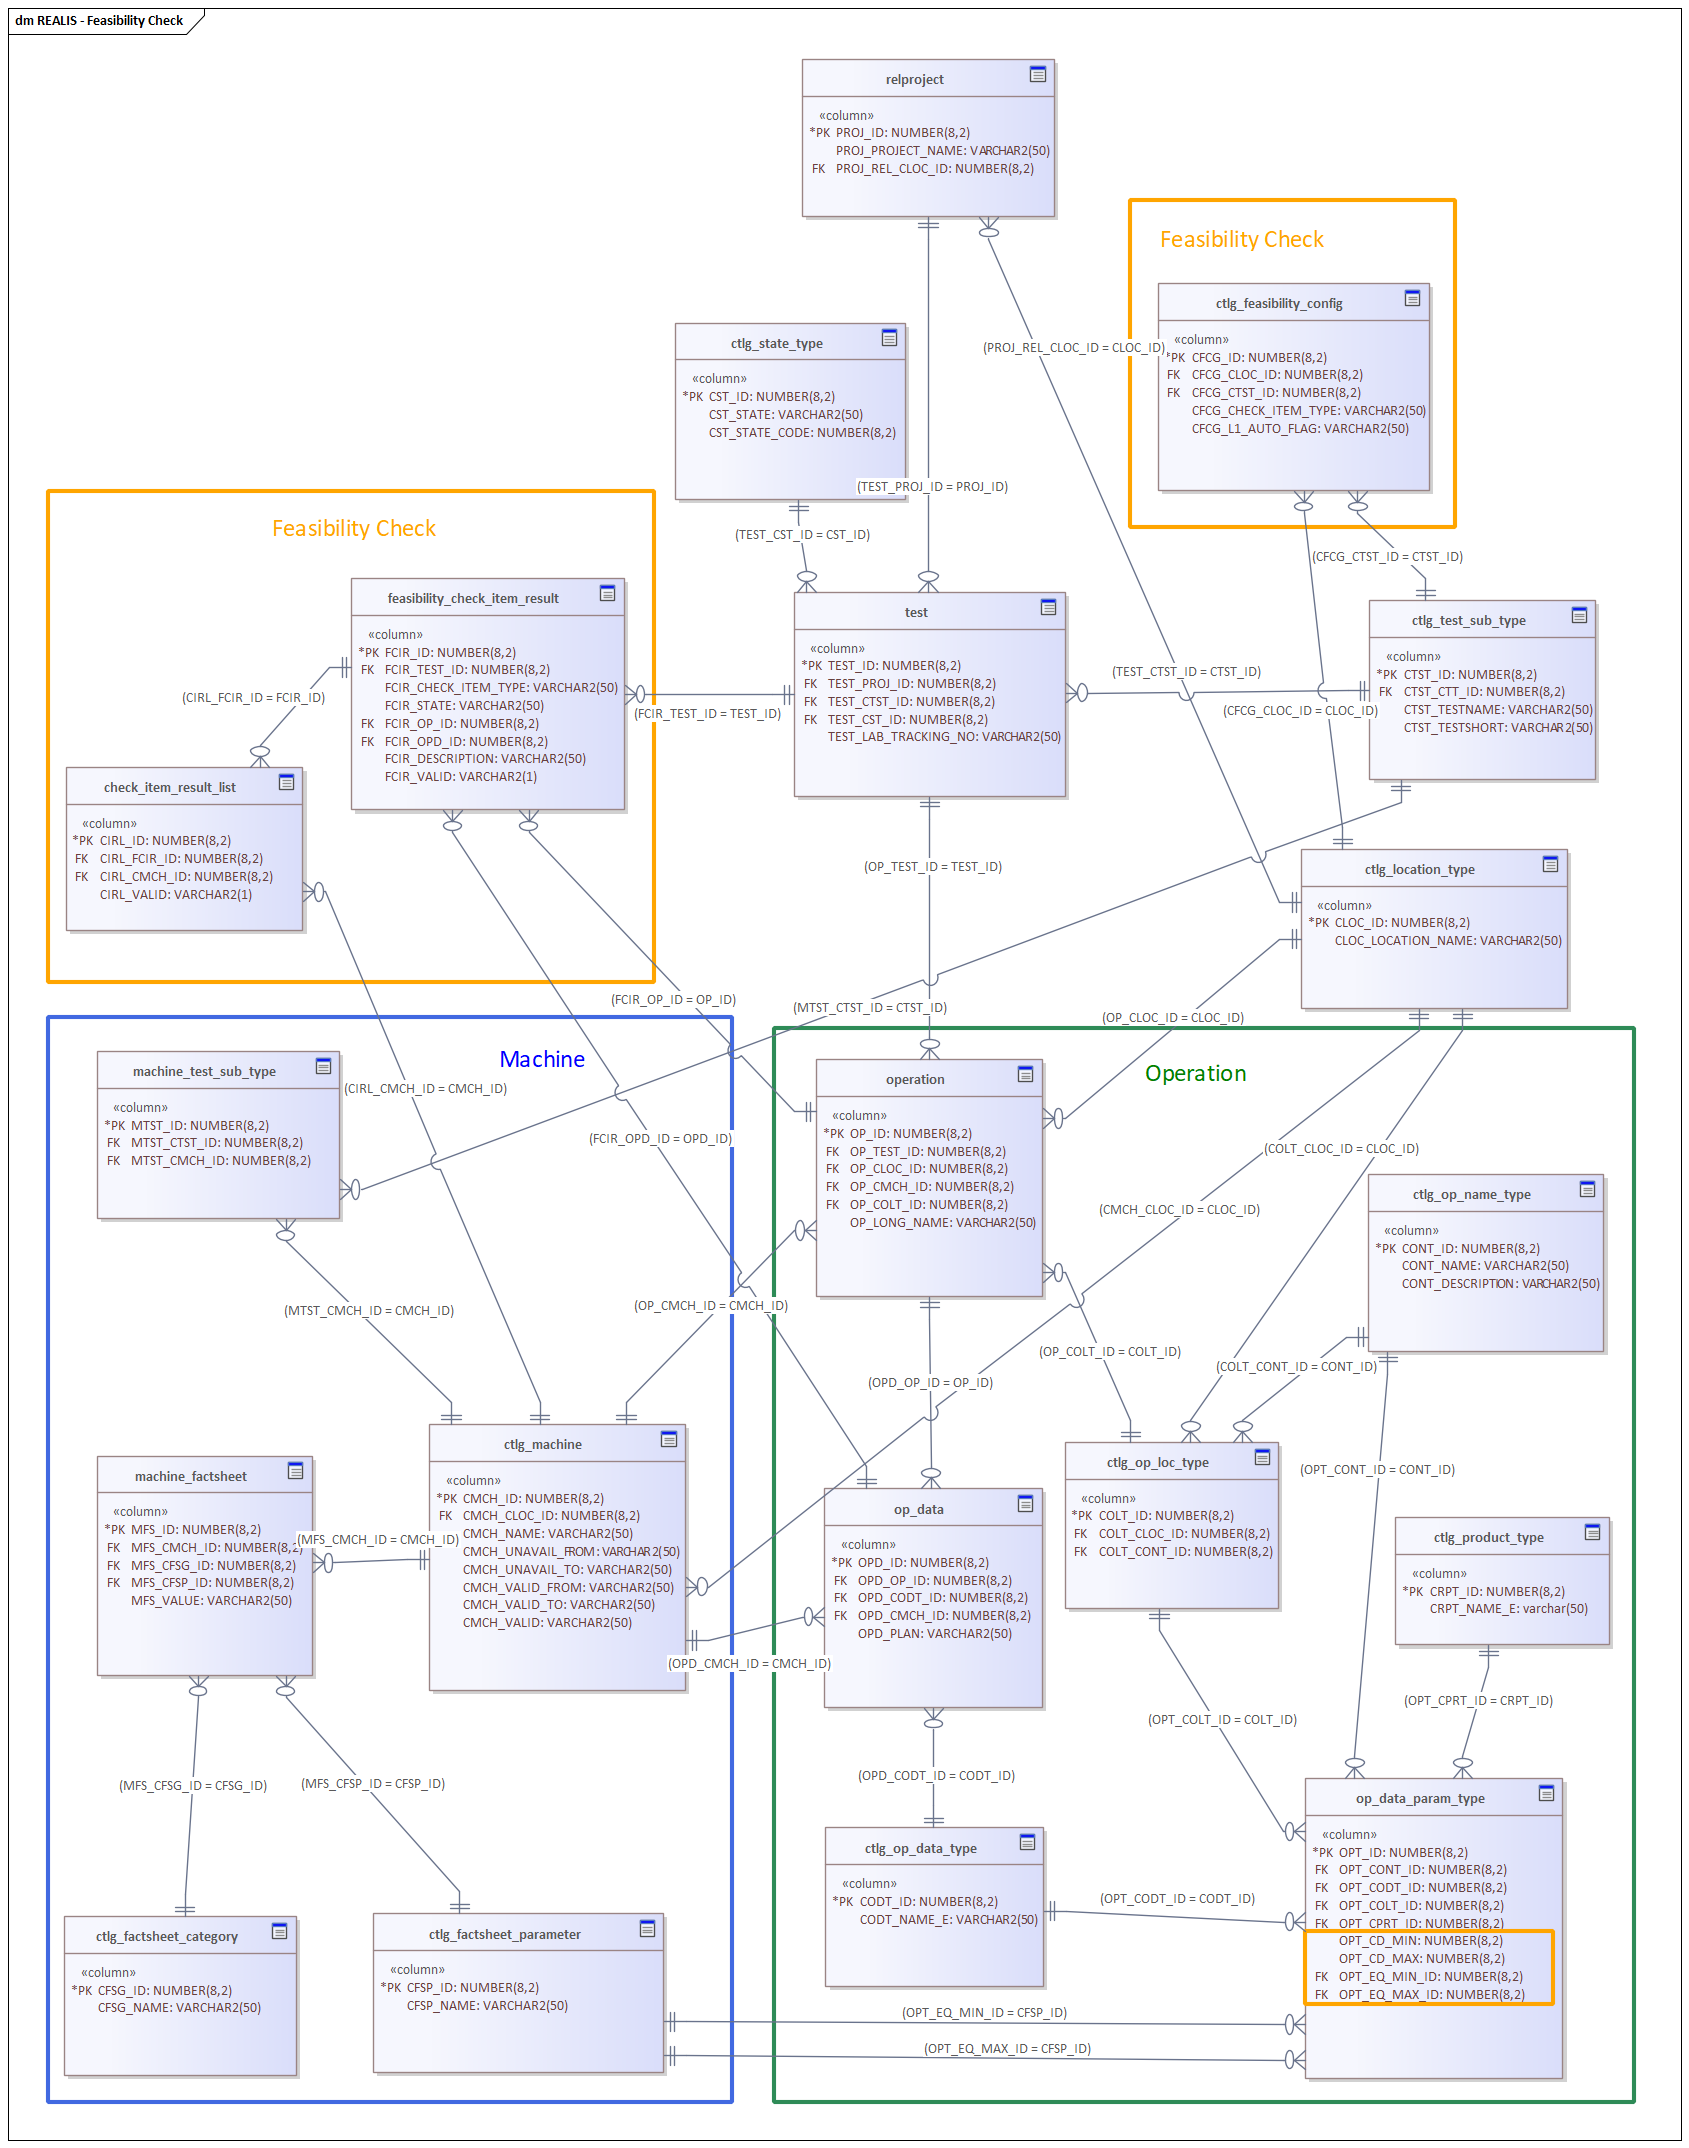
\includegraphics[width=0.98\paperwidth]{bilder/Datenbankdiagramm3.png}}
    \caption{REALIS Datenbankdesign}
    \label{fig:realis-datenbankdesign}
\end{figure}

Die Tabelle \texttt{ctlg\_op\_name\_type} bestimmt welche Arten von Operationen es gibt und legt indirekt über die Tabelle \texttt{ctlg\_op\_loc\_type} fest, welche Operations-Typen in welchen \gls{RPT}-Laboren verfügbar sind. Darüber hinaus definiert die 
\textbf{\texttt{op\_data\_\-param\_type}} Tabelle, welcher Parameter bei welcher Operation in welchem Labor für welche Produkttypen (\texttt{ctlg\_product\_type}) verfügbar ist. Hierbei sind das Labor und der Produkttyp aber nur optionale Einträge, um generische, laborübergreifende und/oder produktübergreifende Einträge zu ermöglichen.

Jeder (Stress-)Parameter einer Operation, der einen konkreten Wert definiert (\texttt{OPD\_\-PLAN}), muss von einer \textbf{Maschine} (\texttt{ctlg\_machine}) umgesetzt werden können. Die eng mit der Maschine verknüpften Tabellen befinden sich in der Abbildung \ref{fig:realis-datenbankdesign} im blau umrandeten Bereich. Eine Maschine ist verknüpft mit einem \textbf{Maschinen-Test-Typen} (\texttt{machine\_test\_sub\_type}), der die Maschine einem Test-Typen (\texttt{ctlg\_\-test\_\-sub\_type}) zuordnet. Des Weiteren besitzen Maschinen verschiedene \textbf{''Fact\-sheets''} (\texttt{machine\_factsheet}) mit einem \textbf{Parameter} (\texttt{ctlg\_\-factsheet\_\-para\-meter}) und einem Wert (\texttt{MFS\_VALUE}). Dieser Wert korrespondiert mit der PlanValue (\texttt{OPD\_\-PLAN}) des Operations-Parameters. 
Er gibt dabei ein Minimum oder ein Maximum der Maschine für diesen Parameter an. Deswegen gibt es (meist) für jeden Operations-Parameter-Typ zwei zugehörige Maschinen-Factsheet-Parameter(-Typen), die anhand ihres jeweiligen Wertes das Minimum und Maximum der Maschine für diesen Parameter festlegen.

Zur besseren Veranschaulichung ein konkretes Beispiel: Ein Temperaturtest besteht aus mehreren Operationen, darunter eine Stressoperation und eine anschließende Funktionsprüfung. Die Stressoperation enthält einen Temperatur-Parameter, dessen \texttt{OPD\_PLAN}-Wert die zu prüfende Testtemperatur definiert (z.B.: 100 °C). Gleichzeitig gibt es spezielle Temperatur-Stress-Maschinen, die über zwei Maschinen-Parameter verfügen: ''Temperatur-Min'' und ''Temperatur-Max''. Diese Parameter besitzen jeweils einen Wert (\texttt{MFS\_VALUE}) und legen darüber gemeinsam die Temperaturspanne fest, innerhalb der die Maschine arbeiten kann.


\subsection{Datenbankerweiterung für Feasibility Check}

Für die Durchführung des Feasibility Checks muss die Datenbank erweitert werden. Dabei sollen die in Kapitel \ref{Subsec:ParameterdestechnischenFeasibilityChecks} beschriebenen Parameter und die zugrunde liegende Logik umgesetzt werden. Zusätzlich müssen die Anforderungen aus Kapitel \ref{Chap:Anforderungen} berücksichtigt werden.

Der Feasibility Check bewertet den Parameter-Wert einer (Stress-)Operation in zwei Dimensionen. Die Überprüfung der \textbf{Sinnhaftigkeit} (\textbf{\gls{ConditionCheck}}) und die Überprüfung der \textbf{Durchführbarkeit} (\textbf{\gls{EquipmentCheck}}).
Dieser Parameter-Wert entspricht in der Datenbank REALIS dem Eintrag \textbf{\texttt{OPD\_PLAN}} in der Tabelle \texttt{op\_data}, die ihn definiert und den Parameter darstellt.

\textbf{\gls{ConditionCheck}} \\
Damit dieser Parameter-Wert auf Sinnhaftigkeit überprüft werden kann, werden in der generischen Verknüpfungs-Tabelle \texttt{op\_data\_param\_type} zwei neue Spalten hinzugefügt. Die Einträge definieren dabei den zulässigen bzw. ''sinnvollen'' Wertebereich für einen Parameter basierend auf den Faktoren: Operationstyp, Parametertyp, Labor und Produkttyp.

\setlength{\leftskip}{1em} 
\textbf{\texttt{OPT\_CD\_MIN}} - definiert die untere Grenze des zulässigen Wertebereichs

\textbf{\texttt{OPT\_CD\_MAX}} - legt die obere Grenze des zulässigen Wertebereichs fest

\setlength{\leftskip}{0em} 

\textbf{\gls{EquipmentCheck}} \\
Für den \gls{EquipmentCheck} wird ebenfalls die Tabelle \texttt{op\_data\_param\_type} um zwei Attribute ergänzt:

\setlength{\leftskip}{1em} 
\textbf{\texttt{OPT\_EQ\_MIN\_ID}} - Referenz auf den minimalen Maschinen-Parameter

\textbf{\texttt{OPT\_EQ\_MAX\_ID}} - Referenz auf den maximalen Maschinen-Parameter

\setlength{\leftskip}{0em} 

Die neuen Spalten dienen als Fremdschlüssel zu zwei Maschinen-Parametertypen (\texttt{ctlg\_factsheet\_parameter}) und ermöglichen die Zuordnung der passenden\linebreak Maschinen zu den jeweiligen Operations-Parametern. Die tatsächlichen Maschinen-\\Parameter-Werte stehen in der verknüpften \texttt{machine\_factsheet}-Tabelle im Feld\linebreak \texttt{MFS\-\_VALUE}. Dadurch lassen sich die Grenzen des umsetzbaren Wertebereichs aller Maschinen für einen spezifischen Operations-Parameter erfassen – eine Funktionalität, die im bisherigen Datenbankmodell von REALIS noch nicht gegeben war.


\textbf{Konfigurierbarkeit des automatisierten Feasibility Checks} \\
Die Konfigurierbarkeit des automatisierten Feasibility Checks legt fest, welche Tests automatisch geprüft werden und welche weiterhin manuell überprüft werden müssen, da manche Tests sich nicht für eine automatische eignen oder andere gar keine Feasibility Check Überprüfung benötigen.

 Dazu wird eine Konfigurationsmöglichkeit in der Datenbank geschaffen. Die Tabelle \textbf{\texttt{ctlg\_feasibility\_config}} ermöglicht die Festlegung, welche Tests automatisiert, manuell oder nicht geprüft werden müssen, abhängig von Labor(-Standort), Test-Typ und CheckItem(-Typ). Ein weiterer Vorteil dieser Konfiguration ist, dass der automatisierte Feasibility Check vor dem vollständigen ''Rollout'' getestet werden kann, indem er gezielt für bestimmte Tests aktiviert wird. Die Spalten der Datenbanktabelle sind in Tabelle \ref{tab:config-fields} erklärt.

\begin{table}[htbp]
    \centering
    \caption{Spalten der Feasibility Check Konfigurations-Tabelle: \texttt{ctlg\_\-feasibility\_\-config}}
    \footnotesize
    \renewcommand{\arraystretch}{1.2}
    \resizebox{\textwidth}{!}{ % Skaliert die Tabelle auf die Seitenbreite
    \begin{tabular}{p{0.3\linewidth} p{0.3\linewidth} p{0.35\linewidth}}
        \toprule
        \textbf{Feldname} & \textbf{Kurzbezeichnung} & \textbf{Beschreibung} \\
        \midrule
        \texttt{CFCG\_L1\_AUTO\_FLAG} & Automatisierungsstatus & Legt fest, ob ein Test automatisiert oder manuell durchgeführt werden soll. \\
        \midrule
        \texttt{CFCG\_CLOC\_ID} & Labor(-Standort) & Berücksichtigt das jeweilige Labor. \\
        \midrule
        \texttt{CFCG\_CTST\_ID} & Test-Typ & Differenzierung nach spezifischen Testarten. \\
        \midrule
        \texttt{CFCG\_CHECK\_ITEM\_TYPE} & CheckItem(-Typ) & Definiert, ob es sich um einen \gls{ConditionCheck} oder einen \gls{EquipmentCheck} handelt. \\
        \bottomrule
    \end{tabular}}
    \label{tab:config-fields}
\end{table}

Falls für eine bestimmte Kombination kein Eintrag in der Konfigurations-Tabelle existiert oder das Automatisierungsstatus-Flag auf \textit{null} gesetzt ist, impliziert dies, dass für diese Verknüpfung kein Feasibility Check erforderlich ist. Diese Regelung ist notwendig, da bestimmte Test-Typen oder Laborstandorte keinen Feasibility Check benötigen. Zudem können bei Einträgen auch die Felder Labor(-Standort), Test-Typ oder CheckItem(-Typ) auf \textit{null} gesetzt werden, um generische Definitionen zu ermöglichen und die Konfiguration flexibler zu gestalten.

\textbf{Speicherung der Feasibilitiy Check Ergebnisse} \\
Die (Teil-)Ergebnisse der durchgeführten Feasibility Checks werden in der Tabelle \textbf{\texttt{feasibility\_check\_item\_result}} gespeichert. Diese ist mit dem jeweiligen Test verknüpft und kann – sofern zutreffend – auch mit hierarchisch tieferliegenden, spezifischeren Ebenen wie der Operation oder einzelnen Parametern assoziiert werden. Diese Verknüpfungen sind jedoch optional, da in manchen Fällen bereits auf Test\-ebene eine abschließende Bewertung möglich ist oder der Test keine spezifischen Operationen und Parameter umfasst.

Jeder einzelne ''Teil-Check'' wird in Abhängigkeit vom jeweiligen CheckItem(-Typ) in der Tabelle abgelegt und umfasst unter anderem die Felder \texttt{FCIR\_STATE}, \texttt{FCIR\_\-DESCRIPTION} und \texttt{FCIR\_VALID}. Dabei dokumentiert \texttt{FCIR\_STATE} den Endstatus des jeweiligen ''Teil-Checks'' (siehe Kapitel \ref{Sec:Backend-Logik} und Abbildung \ref{tab:feasibility-states}), \texttt{FCIR\_DESCRIPTION} liefert eine benutzerfreundliche textuelle Begründung und \texttt{FCIR\_VALID} kennzeichnet, ob das Ergebnis aktuell gültig ist. Da ein Test mehrfach einem Feasibility Check unterzogen werden kann, werden bei jeder neuen Durchführung alle vorherigen Ergebnisse als ungültig markiert, verbleiben jedoch als Historie in der Datenbank.

Die in der Tabelle \texttt{feasibility\_check\_item\_result} gespeicherten Teil-Ergebnisse bilden somit die Grundlage für die Gesamtbewertung eines Tests. Das finale Feasi\-bility-Ergebnis wird aber nicht als einzelner Eintrag gespeichert, sondern durch die Aktualisierung des Teststatus repräsentiert. Anhand der aggregierten Teilergebnisse wird dem Test ein neuer Status zugewiesen: Scheitert mindestens einer der automatisierten ''Teil-Checks'' oder ist eine automatisierte Durchführung nicht möglich bzw. erlaubt, so erhält der Test den neu eingeführten Status ''\textbf{\texttt{MANUALFEASIBILITY}}'', welcher signalisiert, dass eine manuelle Überprüfung erforderlich ist. Werden alle ''Teil-Checks'' hingegen erfolgreich abgeschlossen, so wird der Test auf den bestehenden Status ''\textbf{\texttt{APPLY}}'' gesetzt und damit für den nächsten Schritt im Projekt-Lebenszyklus von REALIS freigegeben. Tritt ein Fehler auf oder bestehen andere Probleme, behält der Test den Status ''\textbf{\texttt{FEASIBILITYREQUESTED}}'', der unmittelbar nach dem Triggern des Feasibility Checks zugewiesen wird.

Wird der Equipment Check erfolgreich abgeschlossen, so werden zusätzlich die Maschinen, die die geforderten Parameter(-Werte) umsetzen können, in der Tabelle \textbf{\texttt{check\_item\-\_result\_list}} hinterlegt. Diese Tabelle stellt eine Verknüpfung zwischen den identifizierten Maschinen und dem entsprechenden Feasibility Check-Ergebnis her.

Durch diese Vorgehensweise wird sichergestellt, dass die detaillierten Teil-Ergeb\-nisse als Grundlage für die finale Testbewertung herangezogen werden, wodurch eine differenzierte und transparente Evaluation der Feasibility Checks möglich ist.







\section{Backend-Logik}

Die Logik des Feasibility-Check-Algorithmus besteht aus vier zentralen Methoden, die zusammen die Prüfung der Machbarkeit eines Tests realisieren. Zum einen gibt es eine Helfer-Methode, die den eigentlichen Algorithmus aufruft und sicherstellt, dass der Aufrufer der REST-API eine aussagekräftige Rückmeldung erhält. Die Kernkomponente bildet die \texttt{FeasibilityCheck()}-Methode, welche abhängig von der Art der Überprüfung den Condition oder den Equipment Check aufruft. Beide Prüfungen sind als eigenständige Methoden implementiert. Der gesamte Ablauf wird durch vier Aktivitäts- bzw. Flussdiagramme visualisiert. In diesen Diagrammen werden Schleifen durch farblich hervorgehobene Bereiche dargestellt, die jeweils einen gleichfarbigen Kreis als Einstiegspunkt sowie einen zweiten als Ausstiegspunkt enthalten.

Die Ausführung des Algorithmus wird initiiert, sobald der Benutzer im Frontend einen \textit{Button} in der Weboberfläche betätigt. Dies löst einen asynchronen HTTP-Call über eine REST-API aus, welcher die Helfer-Methode \texttt{CheckFeasibility()} aufruft und die Test-ID des zu überprüfenden Tests als Argument übergibt.

\begin{figure}[!htbp]
    \centering
    \makebox[\textwidth]{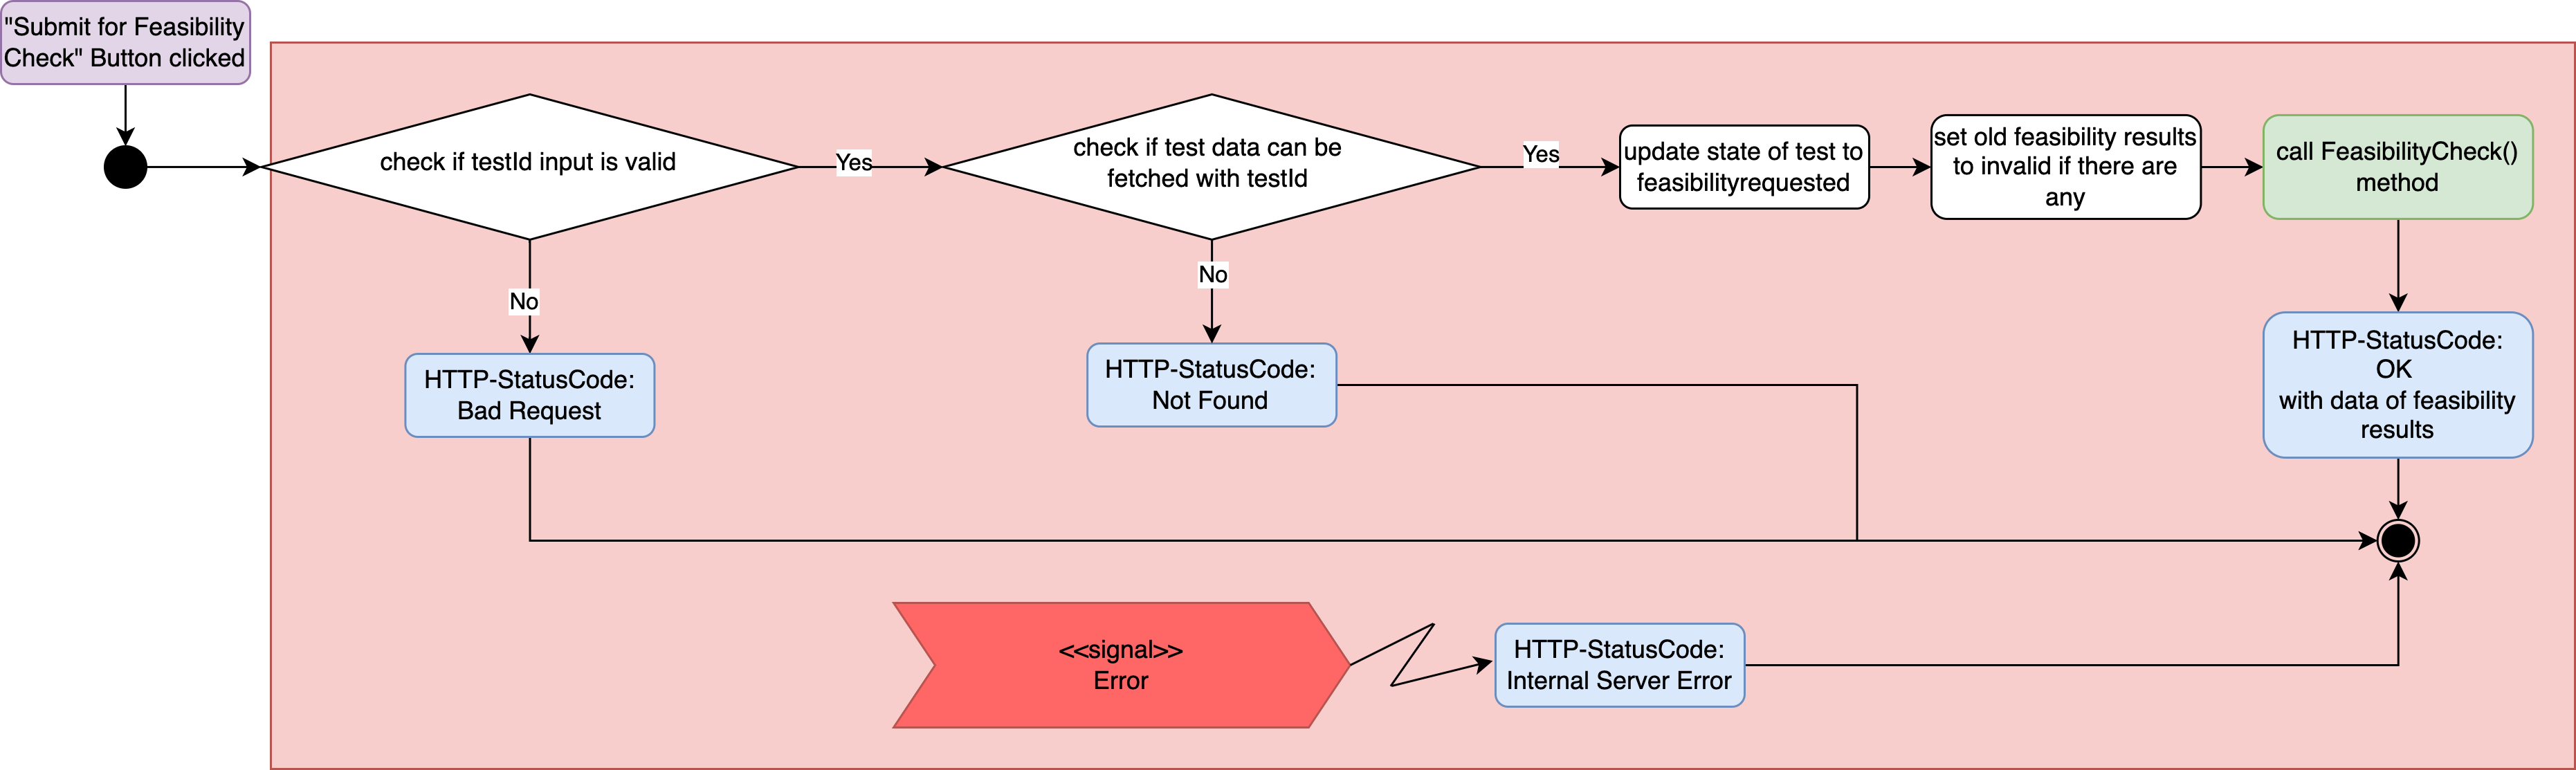
\includegraphics[width=0.85\paperwidth]{bilder/flowchart-check-feasibility-http-call-6-2.png}}
    \caption{Flussdiagramm der Helfer-Methode \texttt{CheckFeasibility()}}
    \label{fig:feasibility-http-call-method}
\end{figure}

Der Ablauf dieser Helfer-Methode ist in Abbildung \ref{fig:feasibility-http-call-method} dargestellt. Ihre Hauptaufgabe besteht darin, die eigentliche \texttt{FeasibilityCheck()}-Methode (grünes Rechteck in der Graphik \ref{fig:feasibility-http-call-method}) auszuführen und gleichzeitig eine geeignete HTTP-Statusmeldung an das Frontend bzw. den Benutzer zurückzugeben. Zusätzlich wird vor der Verarbeitung die übergebene Test-ID auf Gültigkeit überprüft und der Test-Status aktualisiert. Falls der FeasibilityCheck für diesen Test bereits zuvor durchgeführt wurde, werden alte Ergebnisse in der Datenbank als ''invalid'' markiert.


Zur besseren Übersicht wird in Abbildung \ref{fig:feasibility-http-call-method} auch der initiale Button-Klick im Frontend als Aktivität dargestellt. Die eigentliche Logik beginnt jedoch erst nach dem schwarzen Einstiegspunkt, der den Start des Algorithmus kennzeichnet.

\begin{figure}[!htbp]
    \centering
    \makebox[\textwidth]{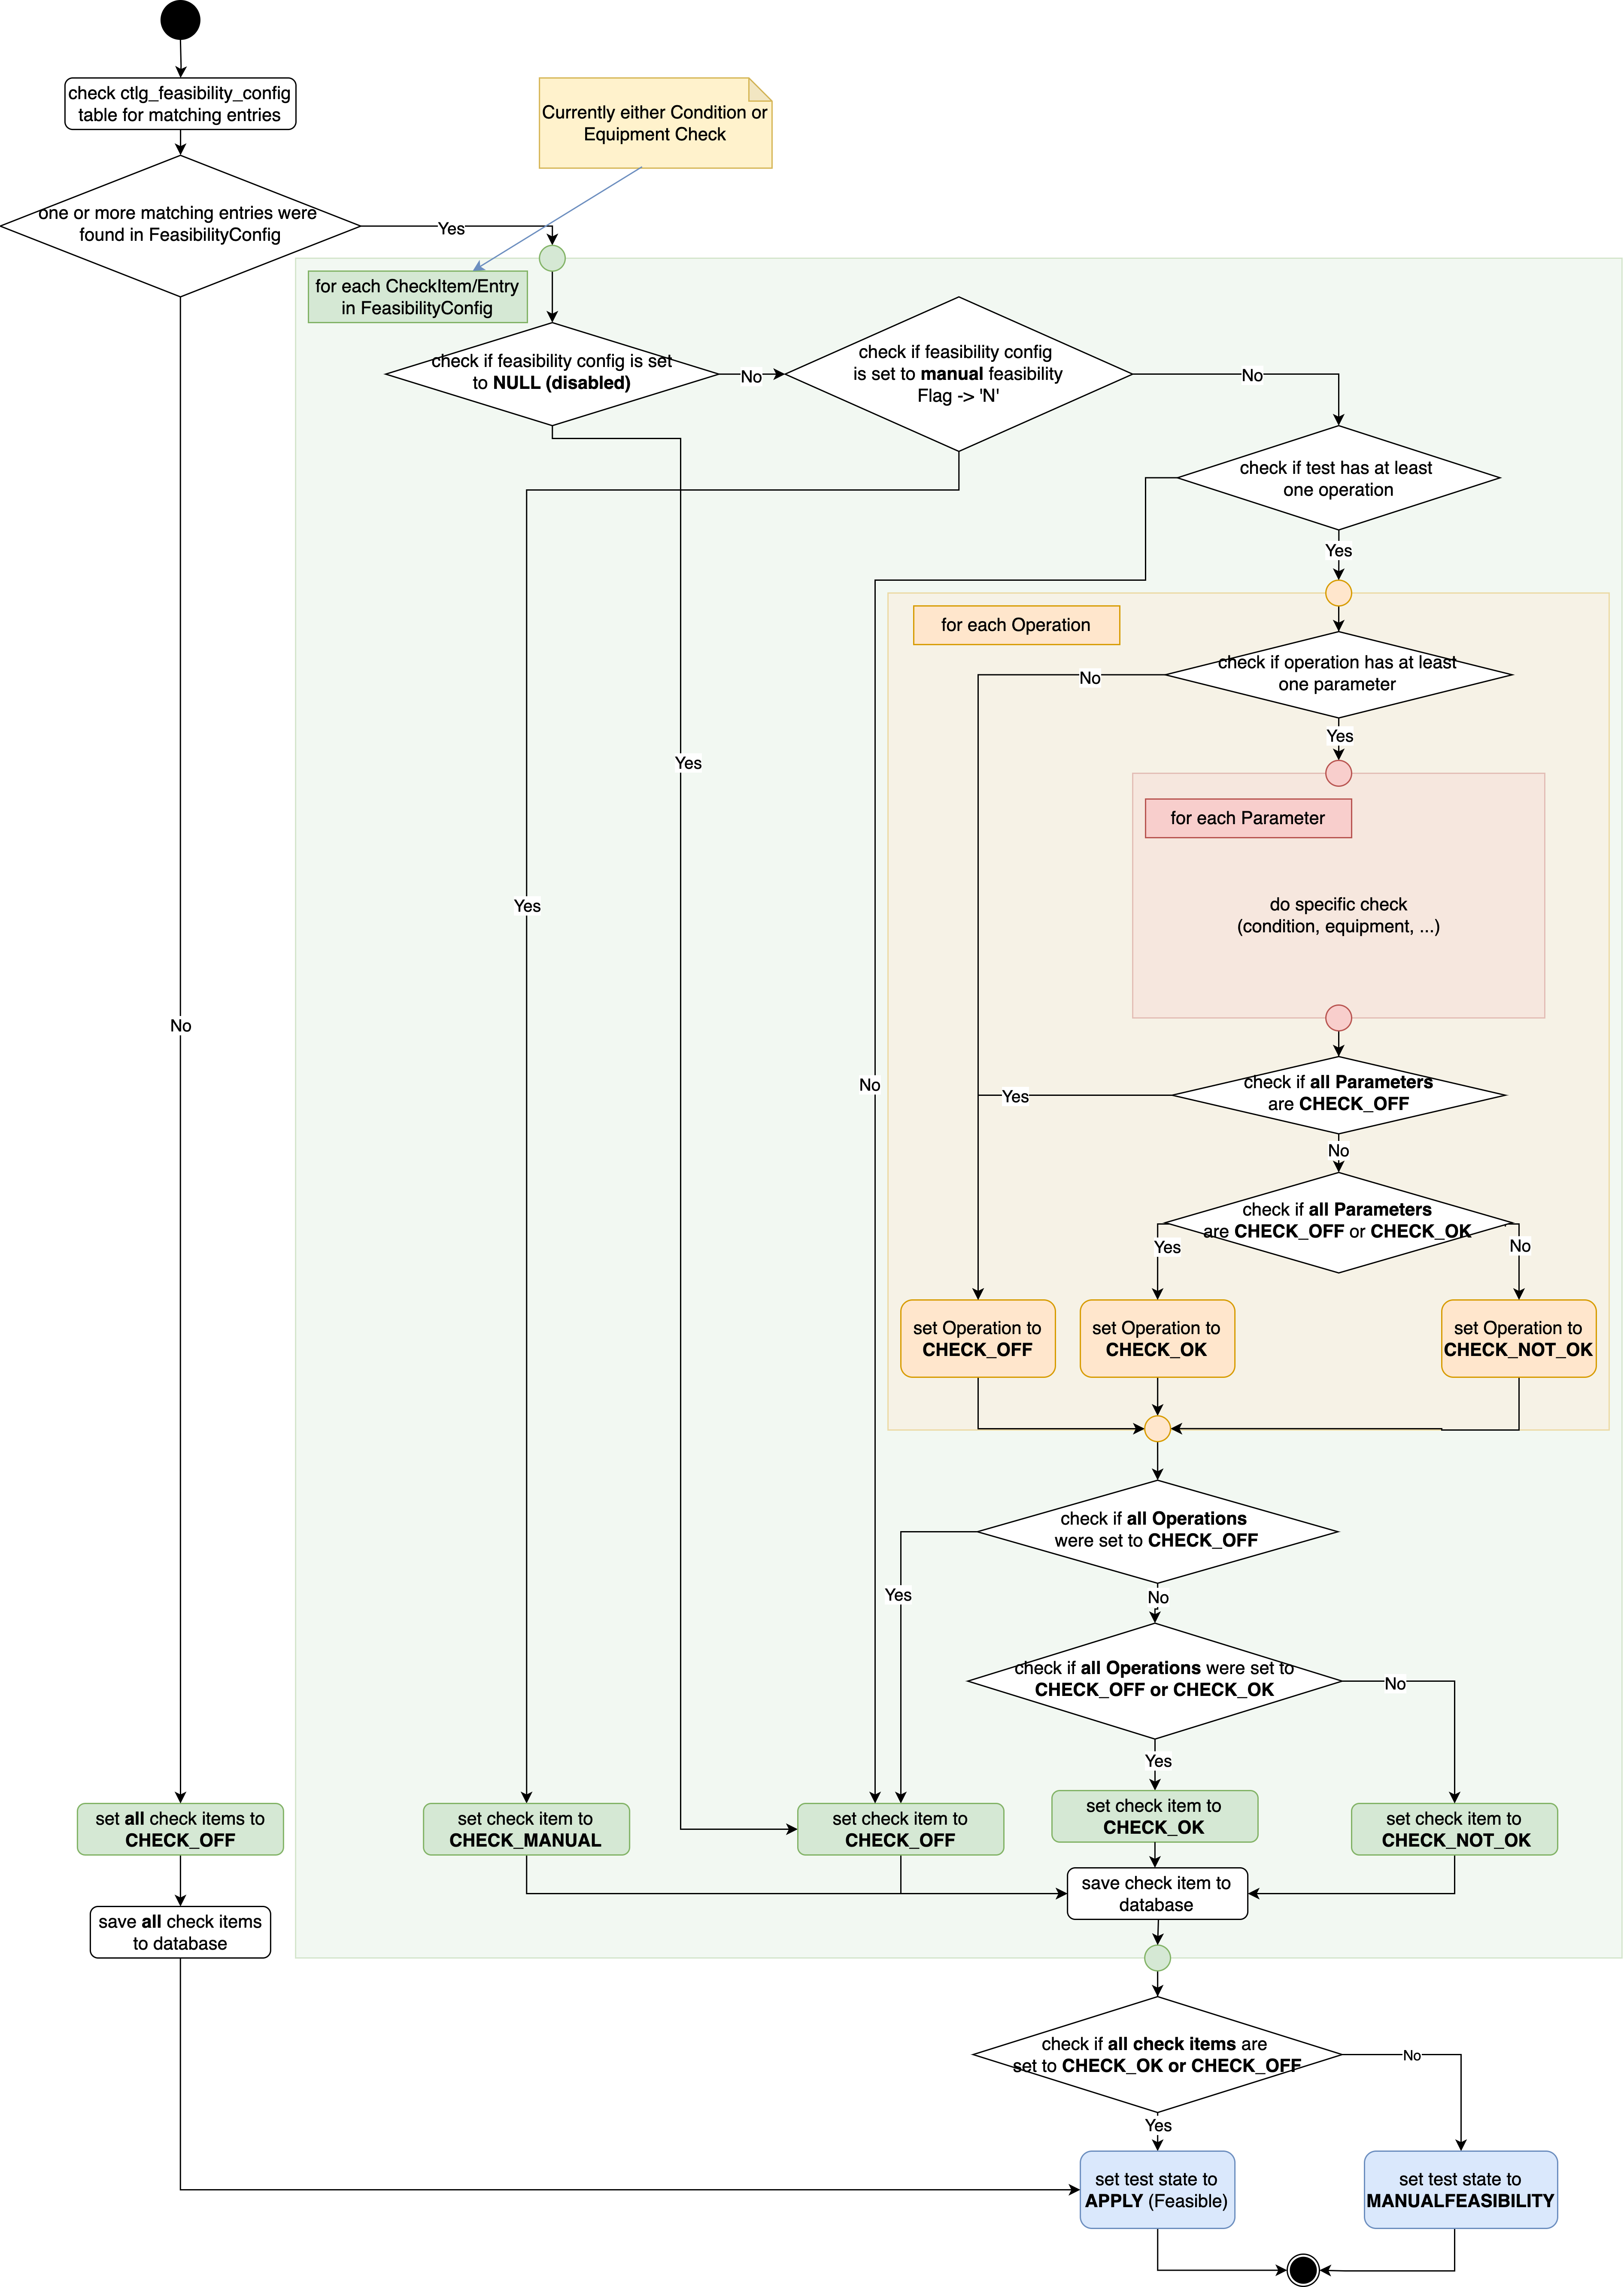
\includegraphics[width=0.85\paperwidth]{bilder/flowchart-feasibilitycheck-modiefied-for-thesis-6-2.png}}
    \caption{Flussdiagramm des Feasibility Check}
    \label{fig:feasibility-check}
\end{figure}

Die Kernlogik des Feasibility Checks wird durch die Methode \texttt{FeasibilityCheck()} ausgeführt, die im Flussdiagramm in Abbildung \ref{fig:feasibility-check} detailliert dargestellt ist. Diese Methode erhält von der Helfer-Methode die Test-ID und überprüft die Machbarkeit des Tests anhand der relevanten Parameter und Operationen. Um die Logik des Algorithmus zu vereinfachen, wird ein Enum eingeführt, das den Status einzelner \textit{Teil-Checks} kennzeichnet. Dieser besteht aus vier möglichen Stati mit jeweils spezifischer Bedeutung:

\setlength{\leftskip}{1em}
\textbf{\texttt{CHECK\_OFF}} - Der Check ist deaktiviert; eine Überprüfung ist weder erforderlich noch vorgesehen. Dies ist insbesondere der Fall, wenn ein Parameter bzw. eine Operation keine Stressoperation darstellt und somit keine PlanValue definiert werden muss.

\textbf{\texttt{CHECK\_OK}} - Der Check war erfolgreich.

\textbf{\texttt{CHECK\_NOT\_OK}} - Der Check war nicht erfolgreich oder es ist ein Fehler aufgetreten.

\textbf{\texttt{CHECK\_MANUAL}} - Eine automatische Überprüfung ist nicht möglich oder der Check ist noch nicht für die automatisierte Überprüfung zugelassen; der Check muss von einem Mitarbeiter manuell durchgeführt werden.

\setlength{\leftskip}{0em} 

Jeder Parameter-Überprüfung wird einer dieser vier Stati zugewiesen. Anschließend wird basierend auf den Statuswerten der einzelnen Parameter ein Gesamtstatus für die zugehörige Operation ermittelt (siehe orange markierte Aktivitäten in Abb. \ref{fig:feasibility-check}). Die Stati aller Operationen ergeben wiederum einen Gesamtstatus für das jeweilige \textit{CheckItem} (\gls{ConditionCheck} oder \gls{EquipmentCheck}) (grüne Aktionen). Dieses Ergebnis dieser Überprüfung wird anschließend als \texttt{feasibility\_check\_item\_result} in der Datenbank gespeichert.

Da die Mehrheit der Ergebnisse den Status \texttt{CHECK\_OFF} aufweist, werden diese nicht in der Datenbank gespeichert, um eine unnötige Datenaufblähung zu vermeiden. Zudem würden in solchen Fällen keine zusätzlichen, für den Benutzer relevanten Informationen generiert werden, da der Status lediglich siganlisiert, dass der Test nicht detailliert überprüft wurde – entweder weil er deaktiviert ist oder weil er keine Operation enthält.

Schließlich wird auf Basis aller \textit{CheckItem}-Ergebnisse der finale Test-Status ermittelt (blaue Aktivitäten). Dieser kann entweder \textbf{''FEASIBLE''} („APPLY“; erfolgreich) oder \textbf{''MANUAL\_FEASIBLE''} (manuelle Überprüfung erforderlich) sein.

Um es zu ermöglichen, dass bestimmte \textit{CheckItems} für einen Test in der Konfiguration vollständig deaktiviert werden können – wobei dies im System als erfolgreiche Überprüfung gewertet wird – kann das entsprechende Flag in der Feasibility-Konfiguration entweder leer (\textit{null}) gelassen werden oder es wird für das betreffende CheckItem gar kein Eintrag in der Konfigurations-Tabelle erstellt. \todo{Beispiel}

\textbf{Konkreter Ablauf des Feasibility Check Algorithmus} \\
Zunächst werden die für den Test hinterlegten Konfigurationen für jedes \texttt{CheckItem} aus der Datenbank abgerufen. Falls kein Eintrag existiert, wird der Check automatisch als erfolgreich gewertet. Ist das zugehörige Flag auf 'N' gesetzt, muss die Überprüfung manuell erfolgen, und der Check ist an dieser Stelle beendet. Nur wenn das Flag auf 'Y' gesetzt ist, wird das entsprechende \textit{CheckItem} (Condition oder \gls{EquipmentCheck}) tatsächlich geprüft.

Anschließend wird überprüft, ob der Test mindestens eine Operation enthält. Falls ja, wird jede dieser Operationen durchlaufen, um festzustellen, ob sie einen oder mehrere Parameter besitzt. Für jeden Parameter wird dann – abhängig vom \textit{CheckItem} – entweder der \gls{ConditionCheck} oder der \gls{EquipmentCheck} durchgeführt.

\subsection{Condition Check}

\begin{figure}[!htbp]
    \centering
    \makebox[\textwidth]{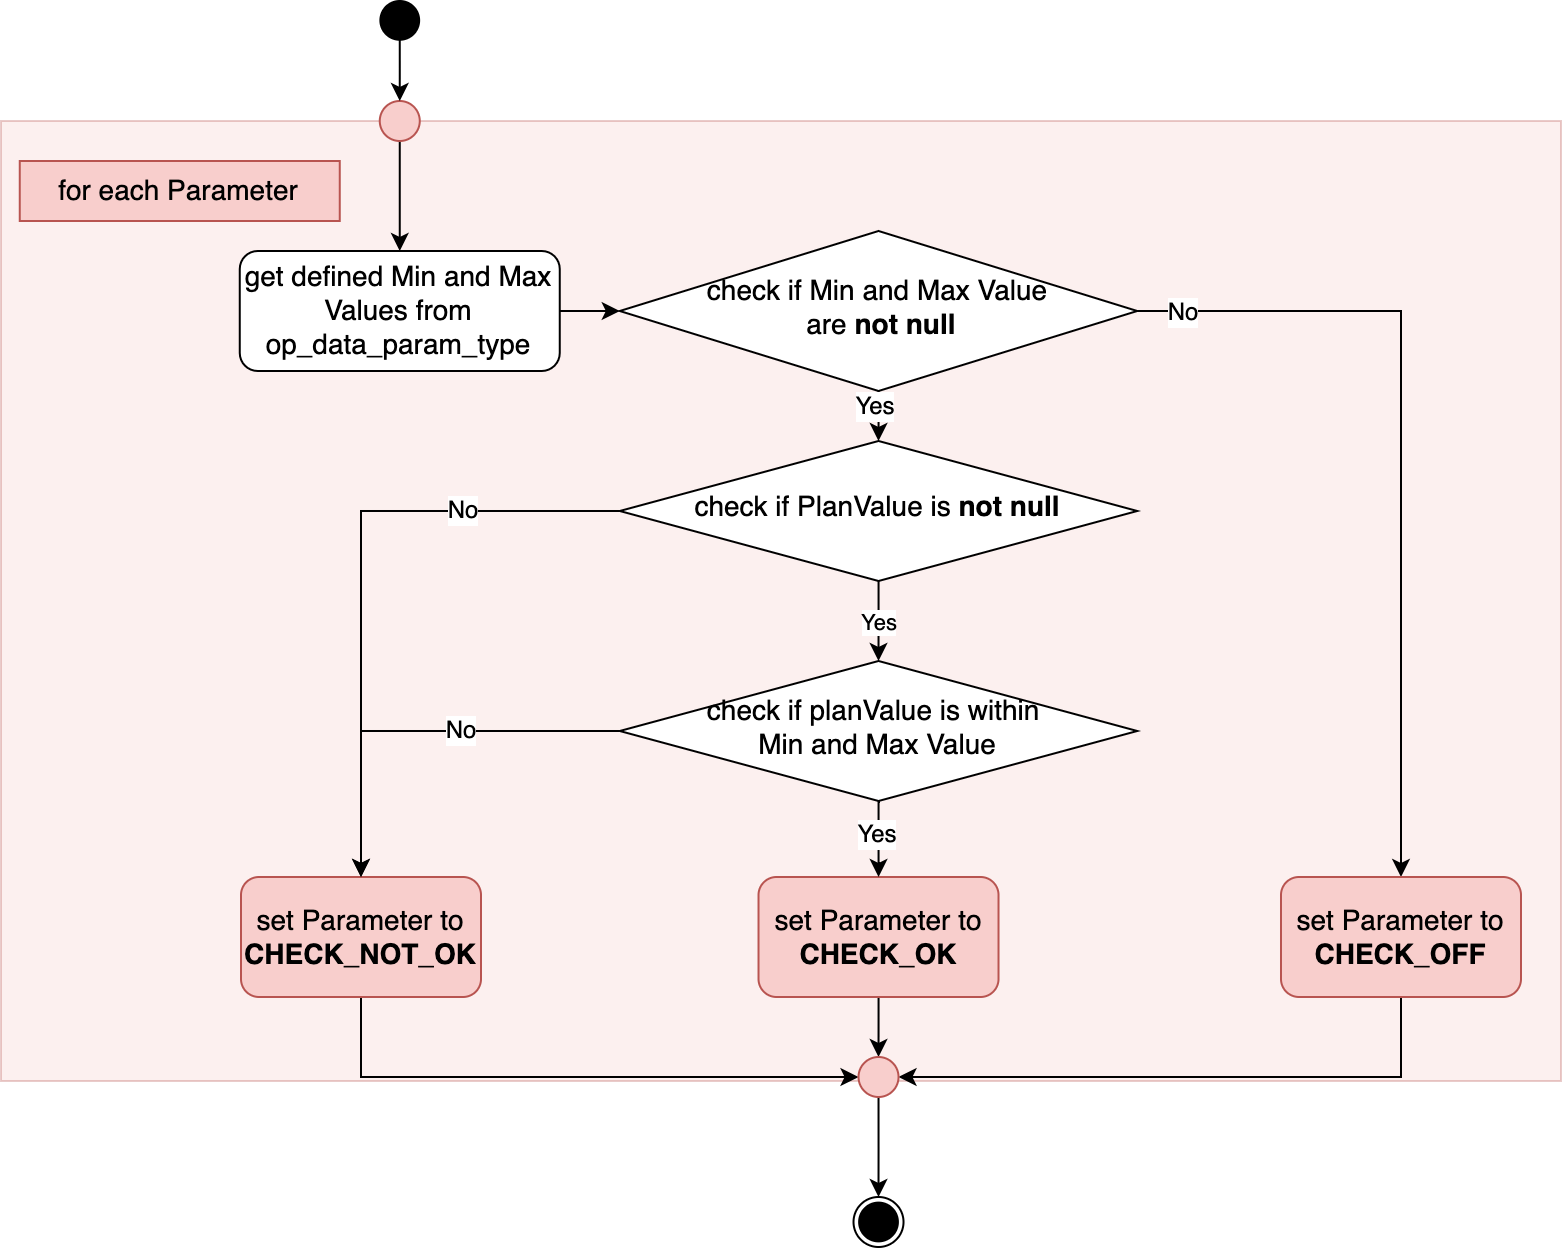
\includegraphics[width=0.80\paperwidth]{bilder/flowchart-condition-check-6-2.png}}
    \caption{Flussdiagramm des \gls{ConditionCheck}s}
    \label{fig:condition-check}
\end{figure}

Der Ablauf des \gls{ConditionCheck} ist in Abbildung \ref{fig:condition-check} dargestellt. Zunächst wird die relevante Verknüpfungstabelle \texttt{op\_data\_param\_type} aus der Datenbank abgerufen. Diese Tabelle definiert den zulässigen Wertebereich eines Parameters durch einen minimalen und maximalen Wert. Falls weder ein minimaler noch ein maximaler Wert definiert ist, wird der \textit{Parameter-Teil-Check} auf \texttt{CHECK\_OFF} gesetzt, was bedeutet, dass keine Überprüfung erforderlich ist und der Parameter automatisch als gültig betrachtet wird. Sind sowohl ein minimaler als auch ein maximaler Wert hinterlegt, muss zusätzlich ein geplanter Wert (\textit{PlanValue}) für den Parameter vorhanden sein. Liegt dieser innerhalb des zulässigen Bereichs, gilt die Sinnhaftigkeitsprüfung als erfolgreich, und der nächste Parameter der Operation wird verarbeitet.


Falls nur ein Mindest- oder Höchstwert in der Datenbank definiert ist, genügt es, wenn der \textit{PlanValue} entweder über dem Mindestwert oder unter dem Höchstwert liegt. Diese Sonderfälle sind zur besseren Übersichtlichkeit nicht im Flussdiagramm \ref{fig:condition-check} dargestellt.




\subsection{Equipment Check}
Der \gls{EquipmentCheck} ist in Abbildung \ref{fig:equipment-check} dargestellt. Der Prozess beginnt ebenfalls mit dem Abruf von Daten aus der passenden \texttt{op\_data\_param\_type} Tabelle. Falls keine Referenzen für den minimalen und maximalen Maschinenparameter (\texttt{ctlg\_factsheet\_parameter}) hinterlegt sind, ist die Überprüfung für diese Parameter, nicht erforderlich und ist somit beendet. Andernfalls muss sichergestellt werden, dass ein \textit{PlanValue} gesetzt ist. Erst danach startet der eigentliche Durchführbarkeits-Check.

Als erstes werden aus der Datenbank alle Maschinen abgerufen, die als ''valide'' gelten, also weder defekt noch in Wartung sind, und zudem den gleichen Testsubtypen aufweisen wie der zu prüfende Test. Die Zuordnung der Maschinen zu einem spezifischen Testsubtyp erfolgt dabei indirekt über die Verknüpfungstabelle \texttt{machine\_test\_sub\_type}, welche die Maschinen mit dem jeweiligen \texttt{ctlg\_test\_sub\_type} verknüpft.

Anschließend werden die verbleibenden Maschinen einzeln durchlaufen (siehe lila markierter Bereich in Abbildung \ref{fig:equipment-check}). Zuerst wird analysiert, ob die Maschine im geplanten Zeitraum der Operation zur Verfügung steht. Danach erfolgt die Überprüfung, ob die Maschine den Parameter grundsätzlich umsetzen kann. Dazu wird geprüft, ob die Maschine über die gleichen \texttt{ctlg\_factsheet\_parameter} verfügt, die in der Verknüpfungstabelle definiert sind. Falls dies der Fall ist, werden die minimalen und maximalen Werte über den zugehörigen Eintrag im Maschinen-Factsheet (\texttt{MFS\_VALUE}) abgerufen. Anschließend wird kontrolliert, ob der geplante Wert (\textit{PlanValue}) des Parameters innerhalb dieser Grenzen liegt. Ist dies der Fall, gilt die Maschine als geeignet, den geplanten Wert umzusetzen, und der Equipment-Check wird als erfolgreich betrachtet.

Alle Maschinen, die den Parameter mit dem geplanten Wert umsetzten können, werden in einer Liste als \texttt{check\_item\_result\_list} erfasst und mit dem zugehörigen \texttt{feasibility\_check\_item\_result} später in der Datenbank abgespeichert. 

\begin{figure}[!htbp]
    \centering
    \makebox[\textwidth]{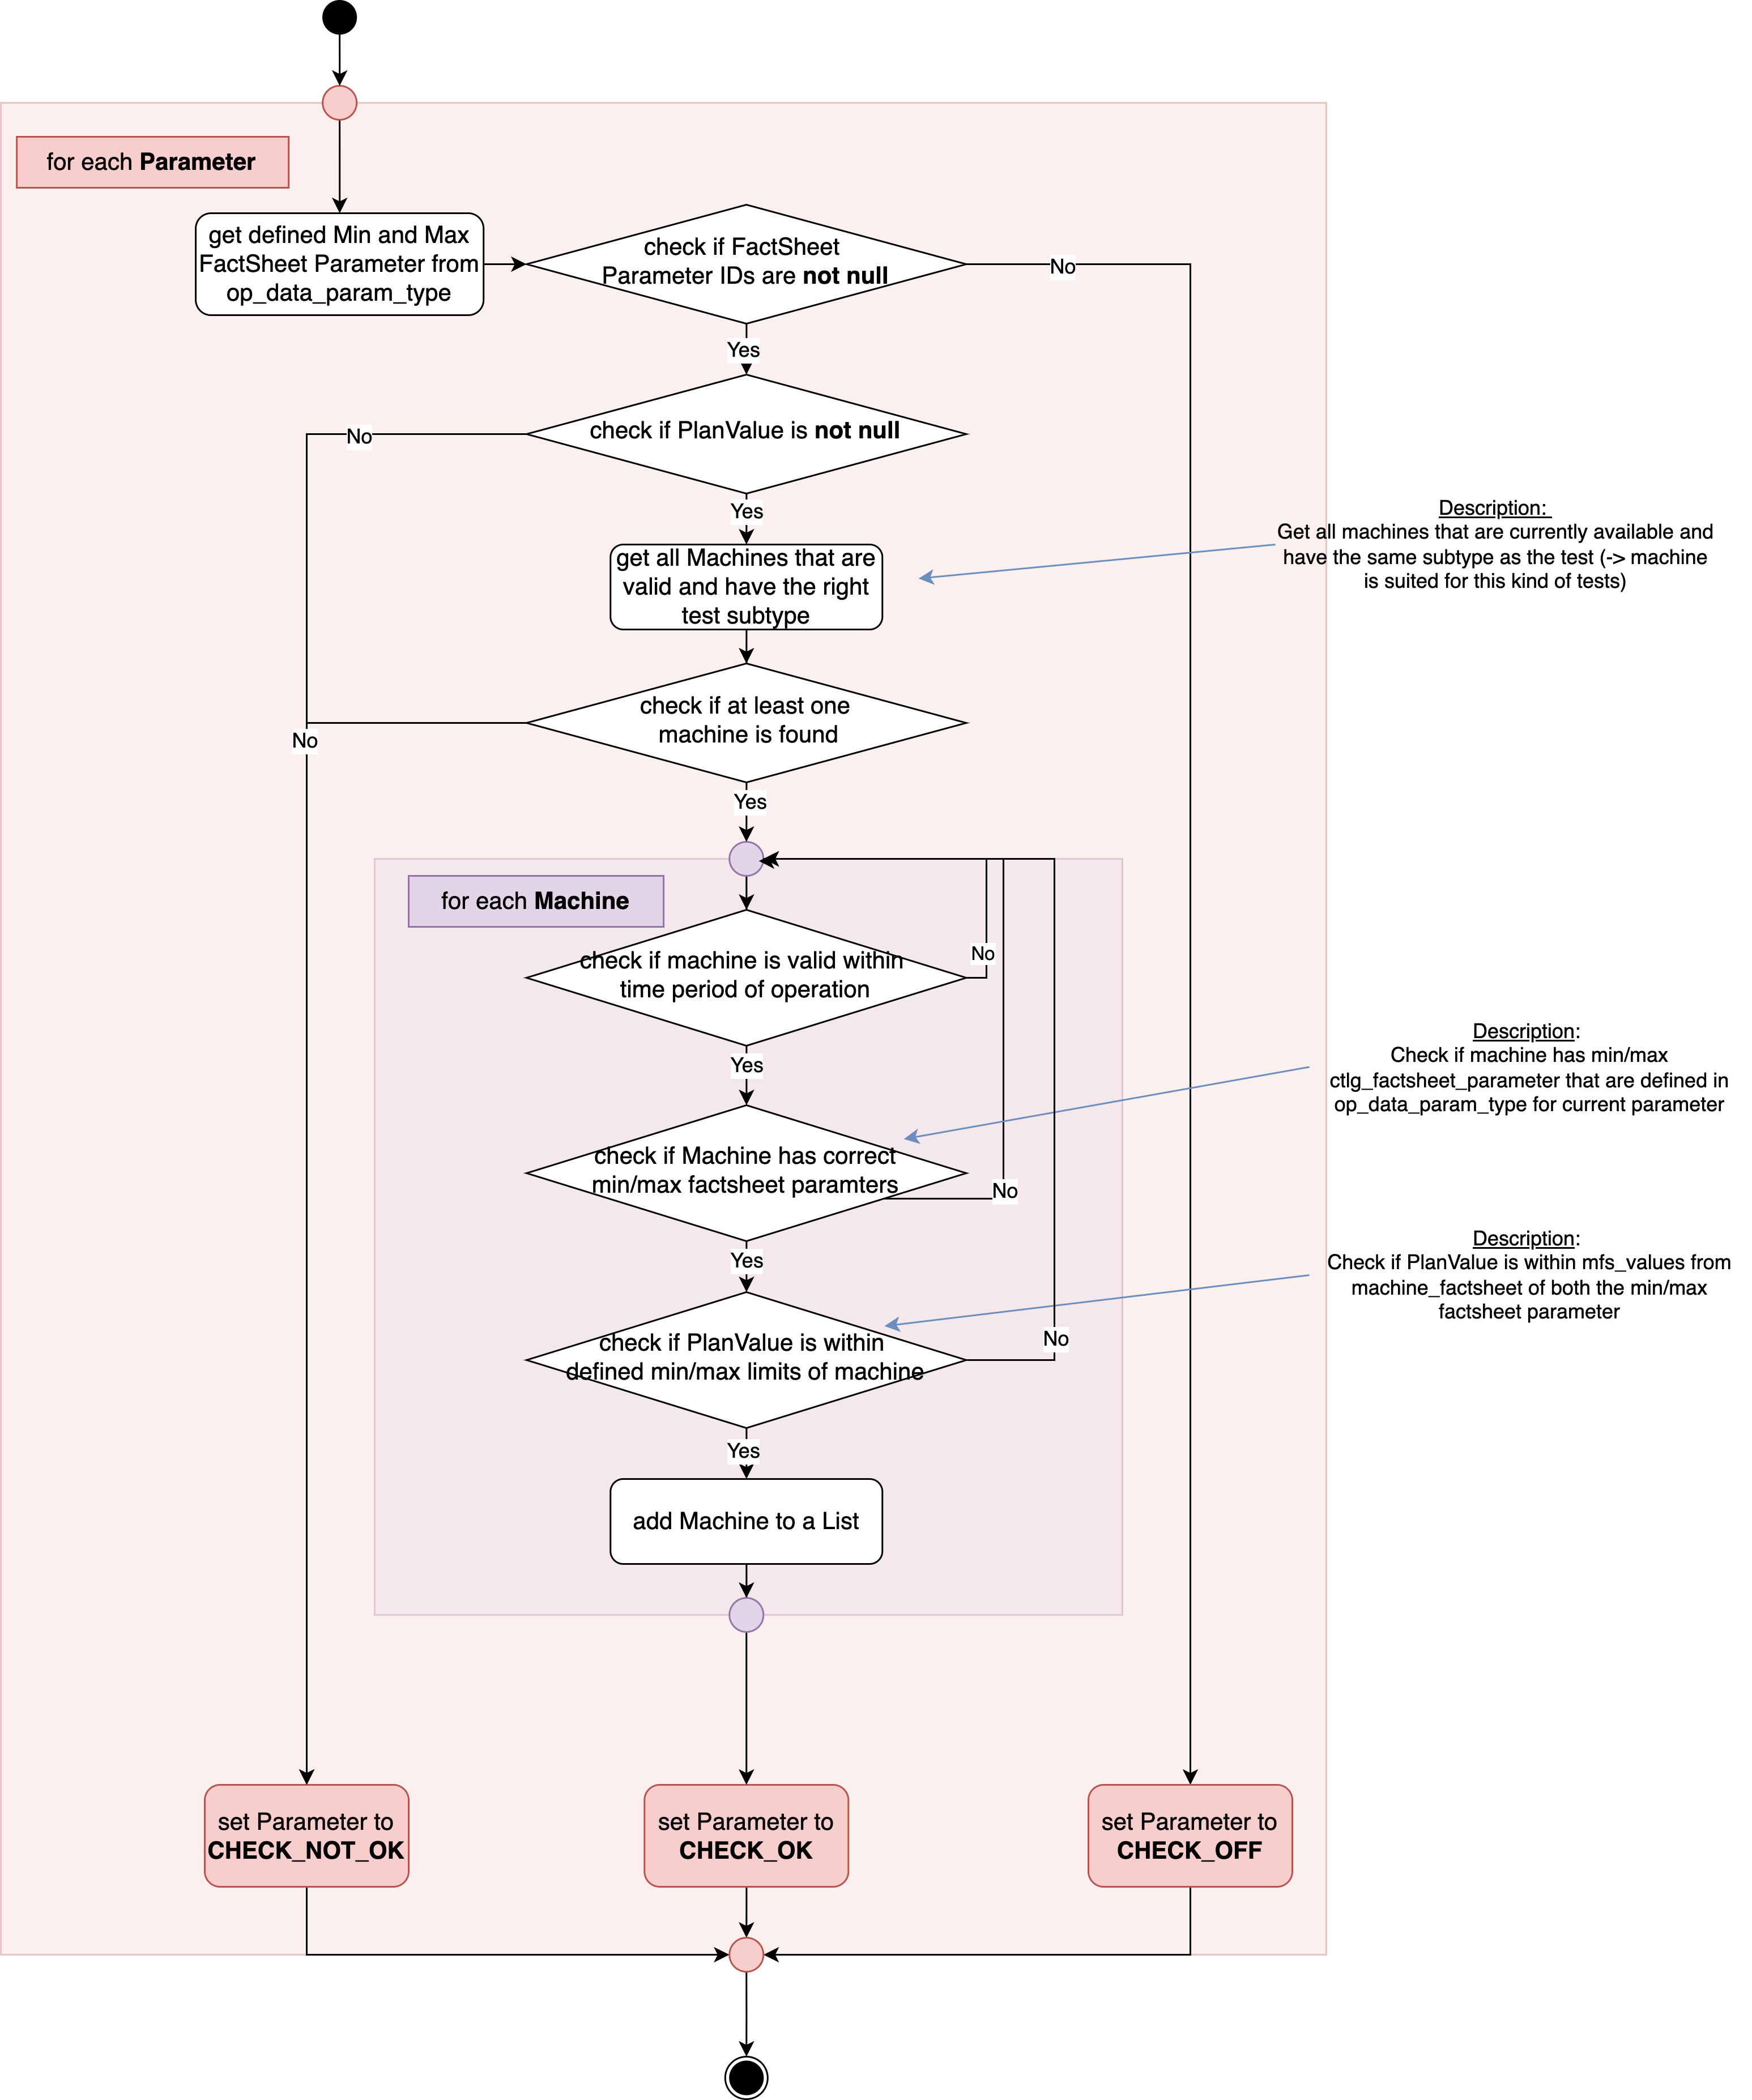
\includegraphics[width=0.85\paperwidth]{bilder/flowchart-equipment-check-6-2.png}}
    \caption{Flowchart des \gls{EquipmentCheck}s}
    \label{fig:equipment-check}
\end{figure}

\section{Frontend-Design}
Das Frontend für den Feasibility Check basiert auf der bereits implementierten Weboberfläche des \gls{REALIS}-Systems. Die Funktionalität des Feasibility Checks wird in die bestehende Webanwendung für den \glsentrylong{QM} integriert, sodass das Projekt nicht mehr an das \gls{RPT}-Labor übergeben werden muss, um den Check durchzuführen. Stattdessen ermöglicht das neue, automatisierte System dem \gls{QM}, die Machbarkeit der angelegten Tests eigenständig und ohne Laborunterstützung zu überprüfen.

Zunächst legt der \glsentrylong{QM} ein neues \gls{REALIS}-Projekt für das zu qualifizierende Produkt an. Dieses Projekt kann mit mehreren unterschiedlichen Tests versehen werden, wobei der Nutzer durch vorgefertigte Templates unterstützt wird, die häufig verwendete Testkonfigurationen und zugehörige Daten enthalten.

Nachdem das Projekt vollständig angelegt wurde, gelangt der Benutzer auf die Weboberfläche, wie in Abbildung \ref{fig:whole-page} dargestellt.

\begin{figure}[!htbp] 
    \centering 
    \makebox[\textwidth]{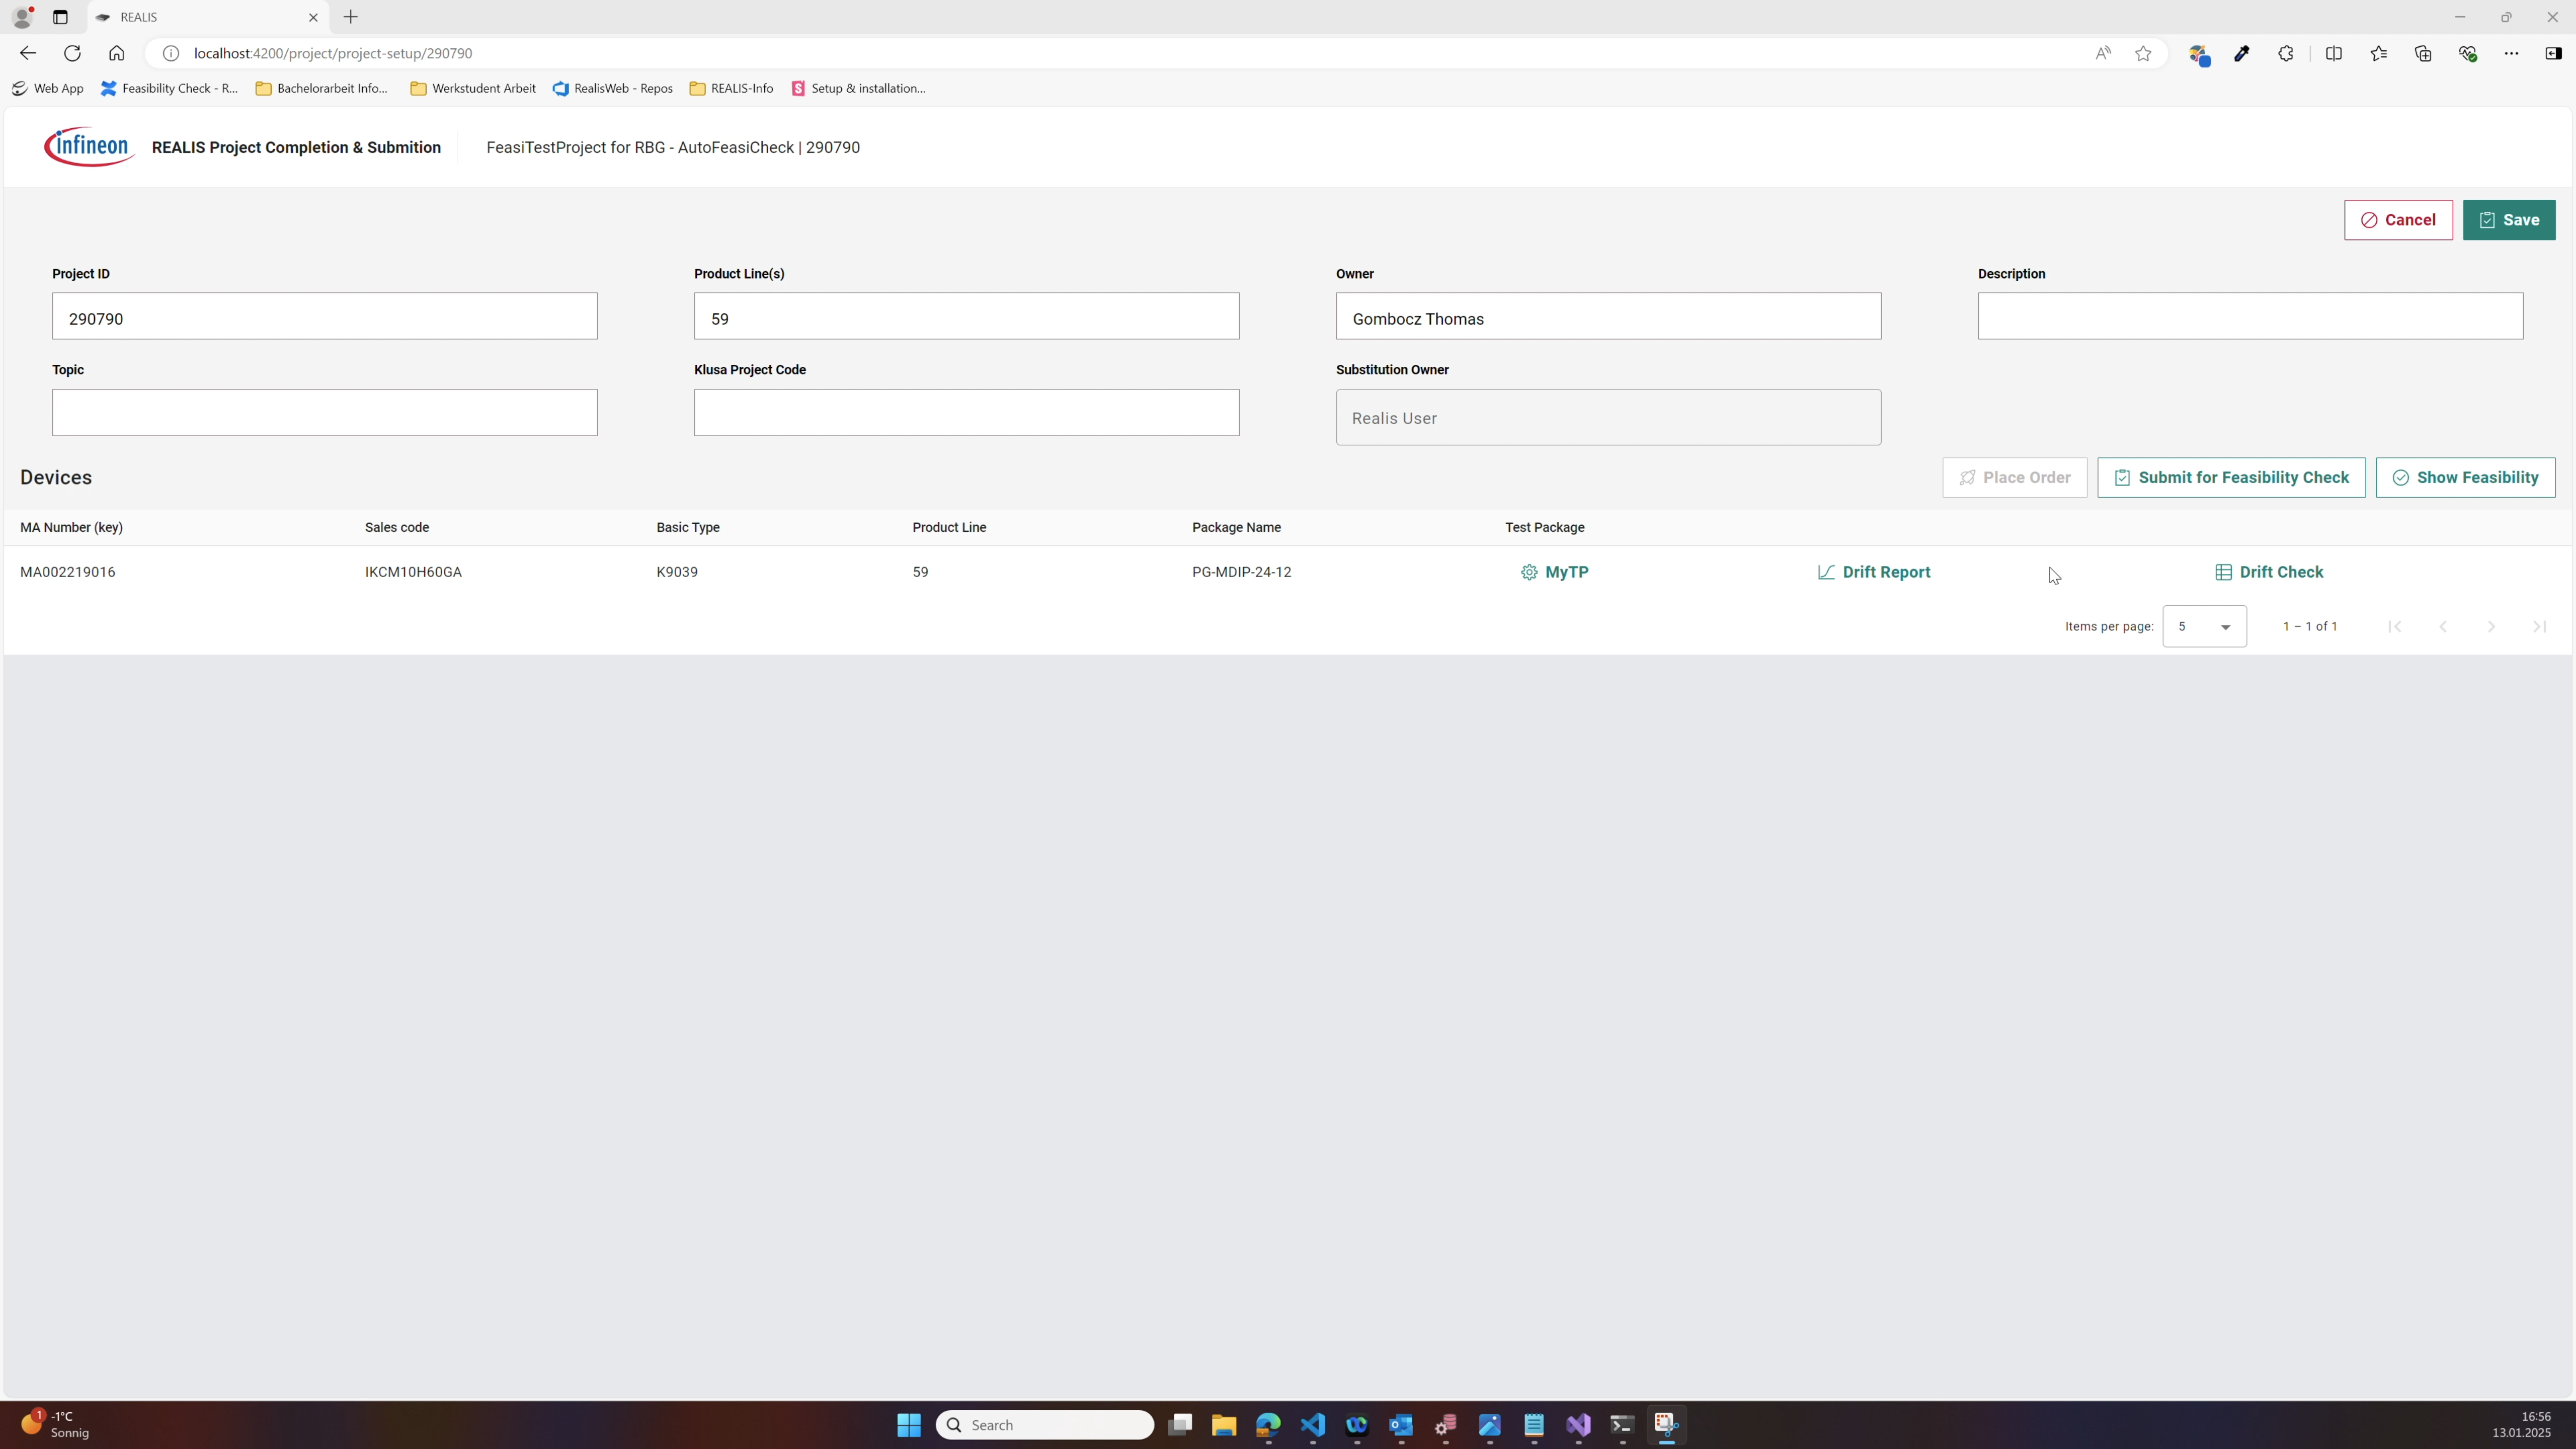
\includegraphics[width=0.85\paperwidth]{bilder/frontend/whole-page.png}} 
    \caption{Weboberfläche für den Quality Manager (QM) – Einstiegspunkt für den Feasibility Check} 
    \label{fig:whole-page} 
\end{figure}

Auf dieser Oberfläche kann der Feasibility Check für die definierten (Stress-)Tests durchgeführt werden. Auf der rechten Seite der Website befindet sich ein grün umrandeter Button mit der Beschriftung "Submit for Feasibility Check". Wird dieser Button betätigt, öffnet sich ein Popup-Fenster (Modal-Page), in dem dem Nutzer eine Übersicht der angelegten Tests in tabellarischer Form präsentiert wird. Diese Tabelle enthält die wichtigsten Informationen, wie den Teststatus und die eindeutige Test-ID (siehe Abbildung \ref{fig:submit-page}).

\subsection{Modal-Page für die Initiierung des Feasibility Checks}

In der Modal-Page können mittels CheckBoxen die einzelnen Tests ausgewählt werden, die den Feasibility Check durchlaufen sollen. Alternativ besteht die Möglichkeit, alle Tests gleichzeitig auszuwählen, indem die oberste CheckBox in der Spaltenüberschriftenleiste aktiviert wird (siehe Mauszeigerposition in Abbildung \ref{fig:submit-page}).

\begin{figure}[!htbp] 
    \centering 
    \makebox[\textwidth]{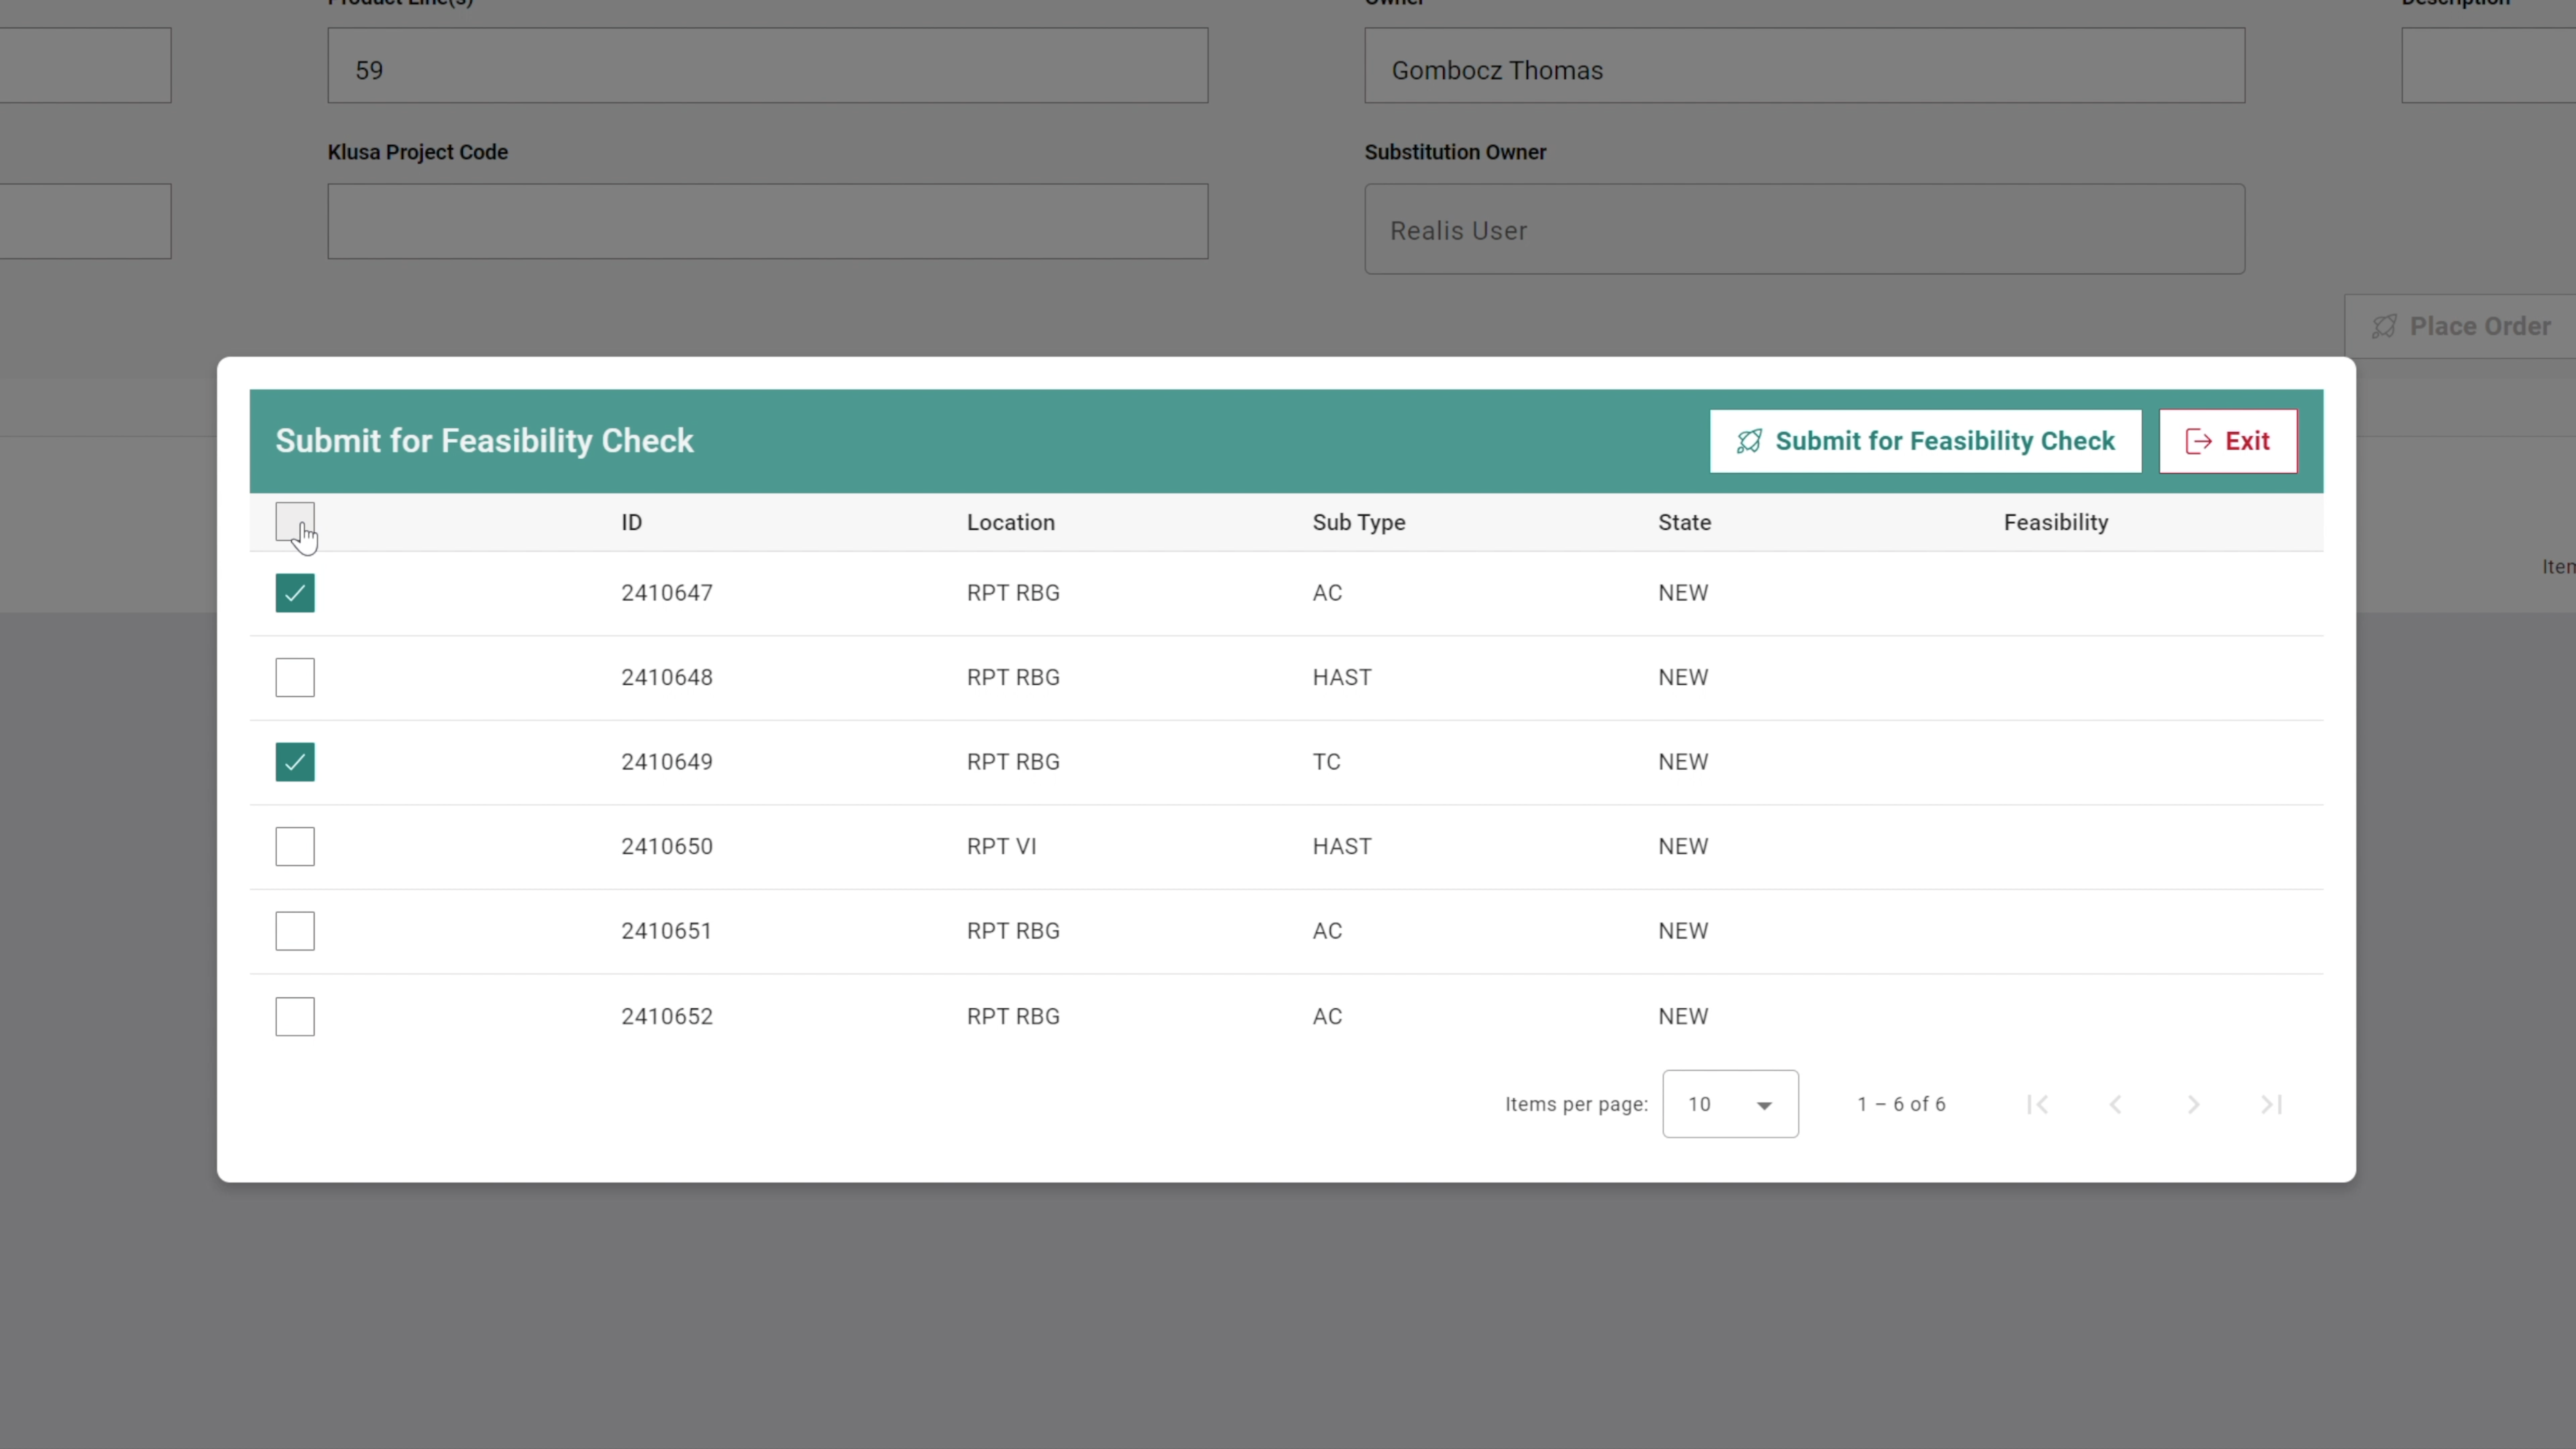
\includegraphics[width=0.85\paperwidth]{bilder/frontend/feasibility-modal-page.png}} 
    \caption{Modal-Page ''Submit for Feasibility Check'' – Modal-Page zur Initiierung des Feasibility Checks} 
    \label{fig:submit-page} 
\end{figure}

Nachdem der Benutzer die gewünschten Tests selektiert hat, klickt er auf den ''Submit for Feasibility Check''-Button, der oben links im Popup, neben dem ''Exit''-Button, positioniert ist. Mit diesem Klick wird für jeden ausgewählten Test ein asynchroner HTTP-Call an die Backend-Logik initiiert. Über die REST-API wird dabei die Helfer-Methode \texttt{CheckFeasibility()} aufgerufen, wobei die jeweilige Test-ID als Parameter übermittelt wird.

Die asynchronen HTTP-Calls ermöglichen es dem Benutzer, weiterhin mit der Oberfläche zu interagieren, während die Überprüfungen im Hintergrund durchgeführt werden. Dadurch kann der Benutzer das Popup schließen oder andere Aktionen ausführen, ohne den laufenden Feasibility Check zu unterbrechen. Die rotierenden Ladekreise in der "Feasibility"-Spalte rechts veranschaulichen den Ladevorgang für den Feasibility Check jedes Tests (siehe Abbildung \ref{fig:loading-with-results}). Bis ein Resultat eintrifft vergehen circa 2 bis 15 Sekunden, je nach Feasibility-Konfiguration und Komplexität des Tests.

\begin{figure}[!htbp] 
    \centering 
    \makebox[\textwidth]{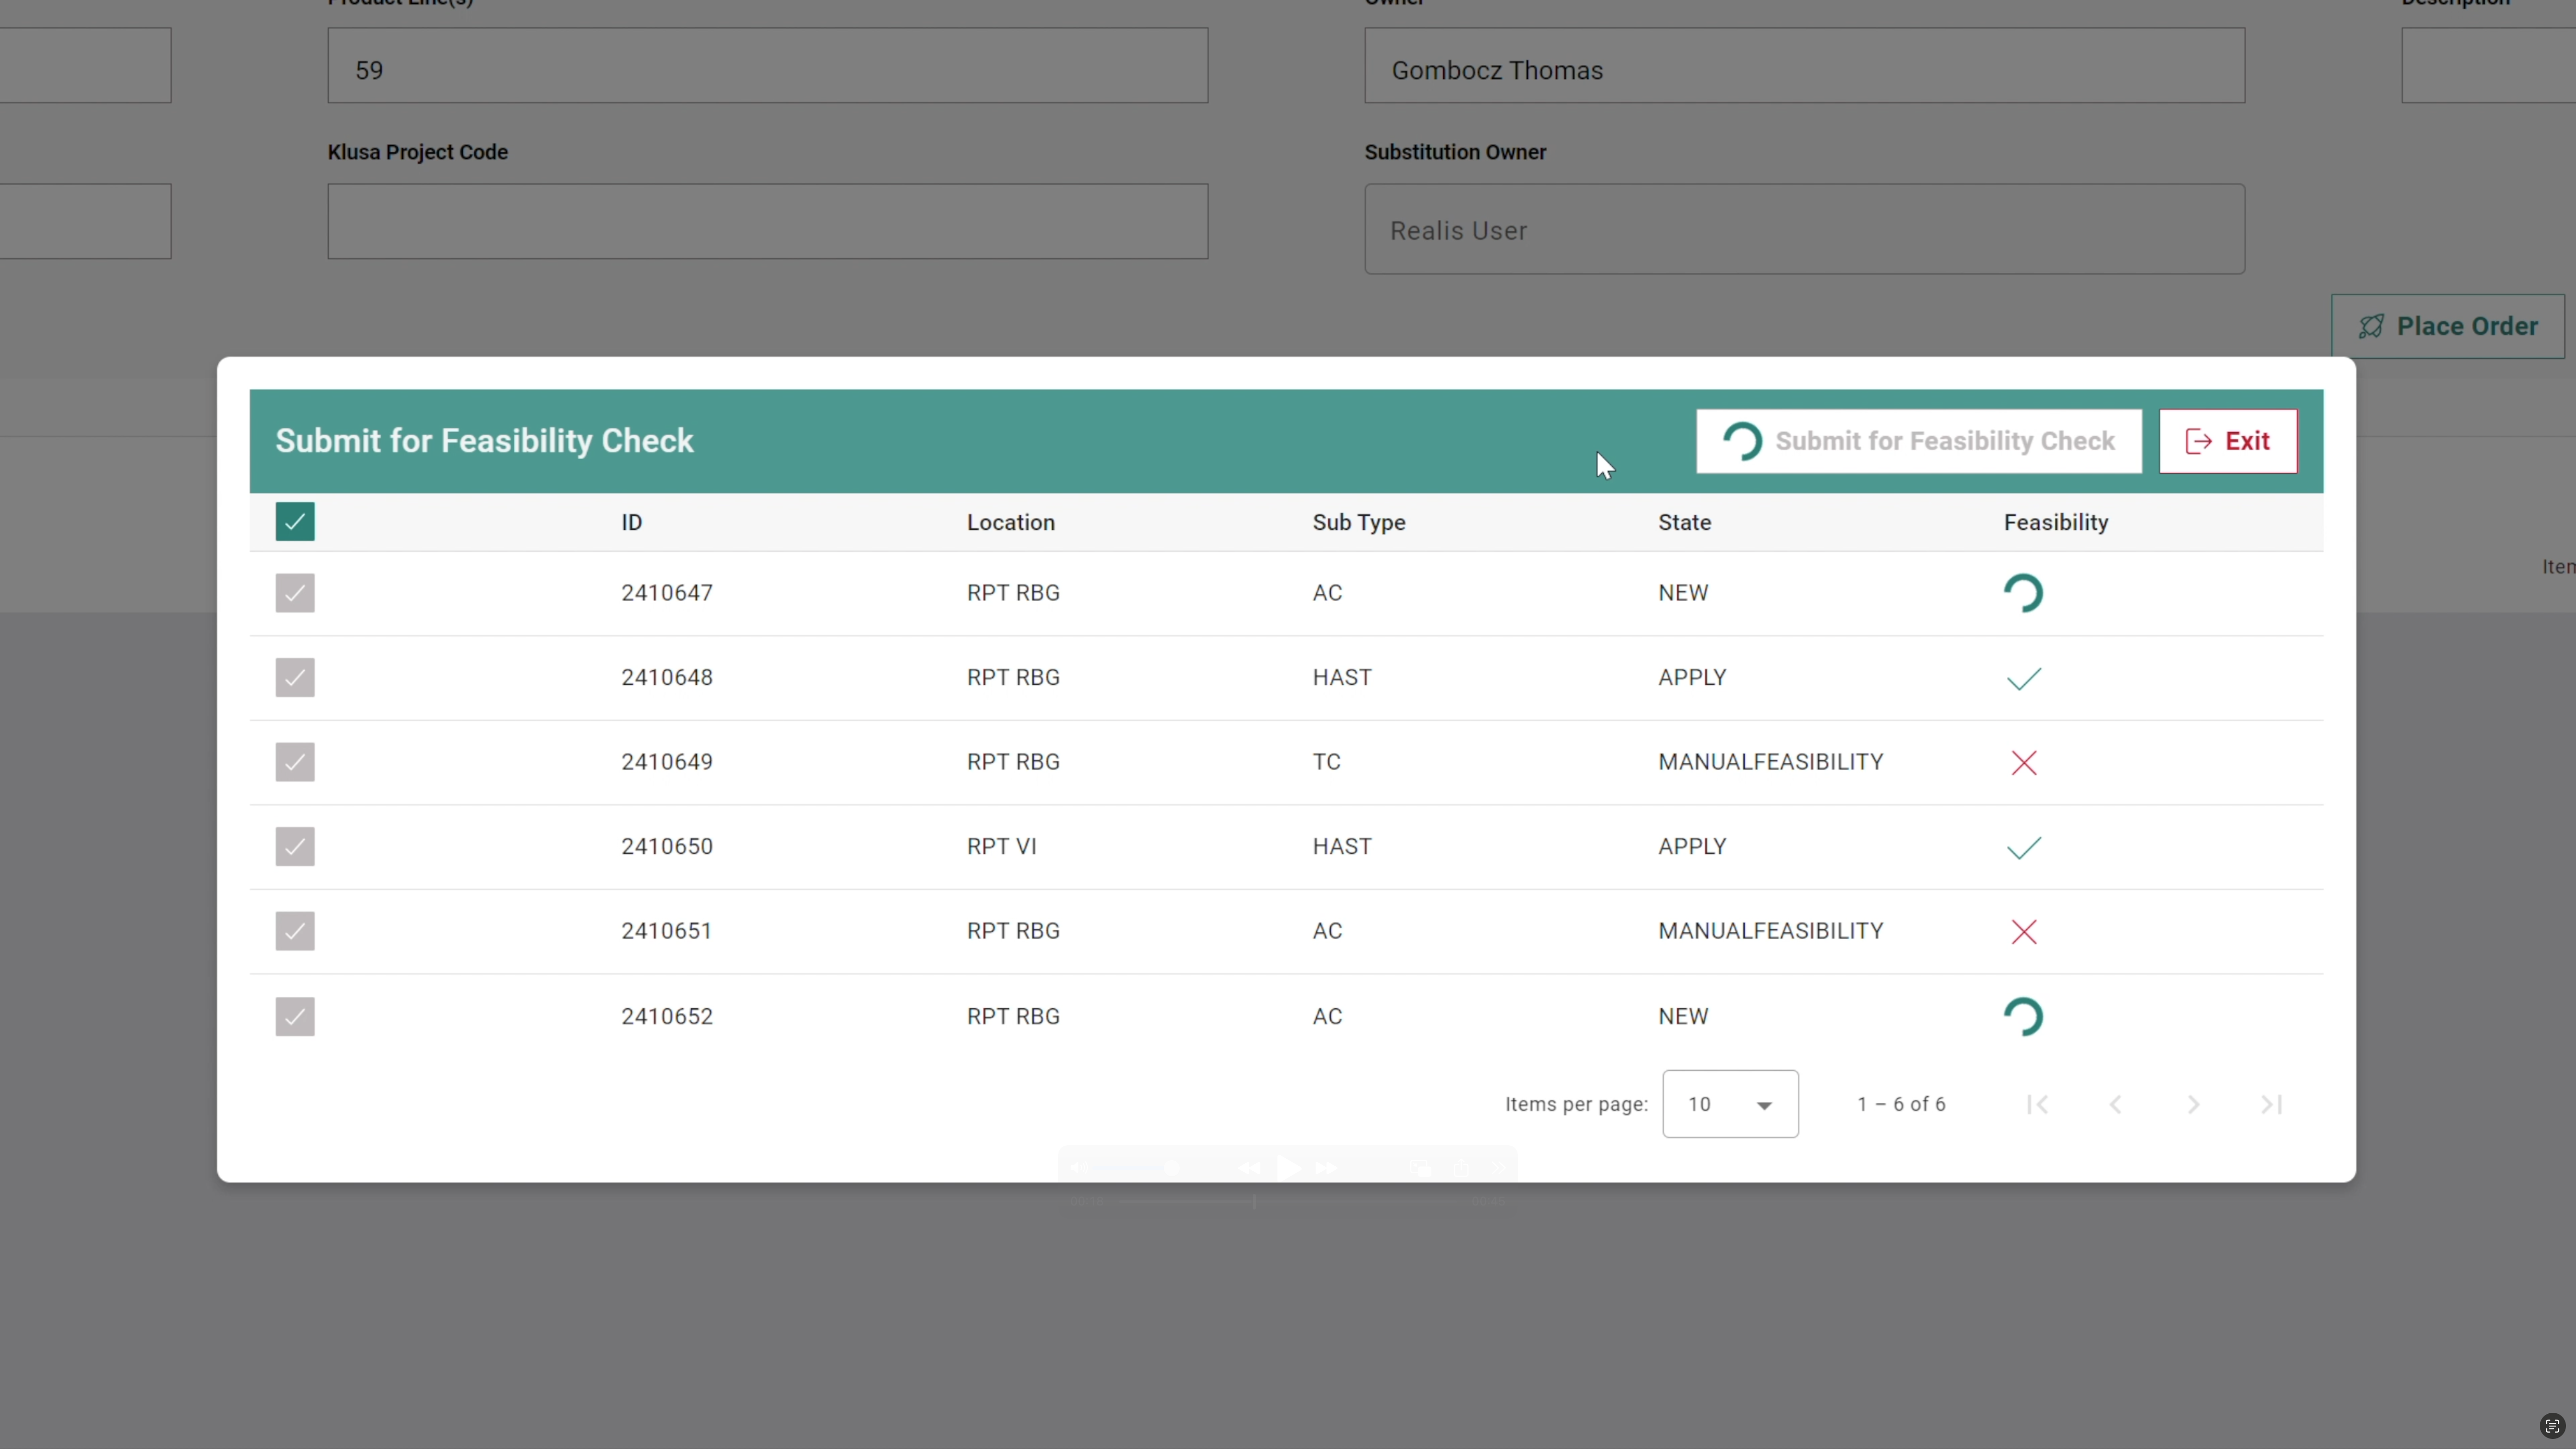
\includegraphics[width=0.85\paperwidth]{bilder/frontend/loading-with-results.png}} 
    \caption{Modal-Page ''Submit for Feasibility Check'' – Ladevorgang und erste Ergebnisse} 
    \label{fig:loading-with-results} 
\end{figure}

Sobald die ersten Überprüfungen abgeschlossen sind, verschwindet der Ladekreis. Anschließend werden drei Icons angezeigt und der Test-Status in der Tabelle aktualisiert.

Ein grüner Haken zusammen mit dem Status ''APPLY'' (bzw. „FEASIBLE“) signalisiert, dass der Feasibility Check erfolgreich war.

Ein rotes Kreuz und der Status ''MANUALFEASIBILITY'' weisen darauf hin, dass entweder ein oder mehrere Kriterien nicht erfüllt wurden oder der Test in der Konfiguration noch nicht für die automatisierte Überprüfung freigeschaltet ist. In beiden Fällen muss der Test manuell von einem Mitarbeiter überprüft werden.

Tritt ein Fehler im Algorithmus auf, erscheint ein rotes Dreieck mit Ausrufezeichen. In diesem Fall bleibt der Test-Status unverändert oder wird auf ''FEASIBILITY\_REQUEST'' gesetzt, je nachdem wann und welcher Fehler auftritt (dieser Fall ist in der Abbildung \ref{fig:loading-with-results} nicht dargestellt).


\subsection{Modal-Page für detaillierte Ergebnisse des Feasibility Checks}

Nachdem der Feasibility Check für einige Tests abgeschlossen ist, können in einer zweiten Modal-Page detaillierte Ergebnisse eingesehen werden. Diese Seite wird geöffnet, wenn der Benutzer den grün umrandeten „Show Feasibility“-Button in der Startoberfläche (siehe Abbildung \ref{fig:whole-page}) betätigt. Abbildung \ref{fig:result-details} zeigt diese Modal-Page.

\begin{figure}[!htbp] 
    \centering 
    \makebox[\textwidth]{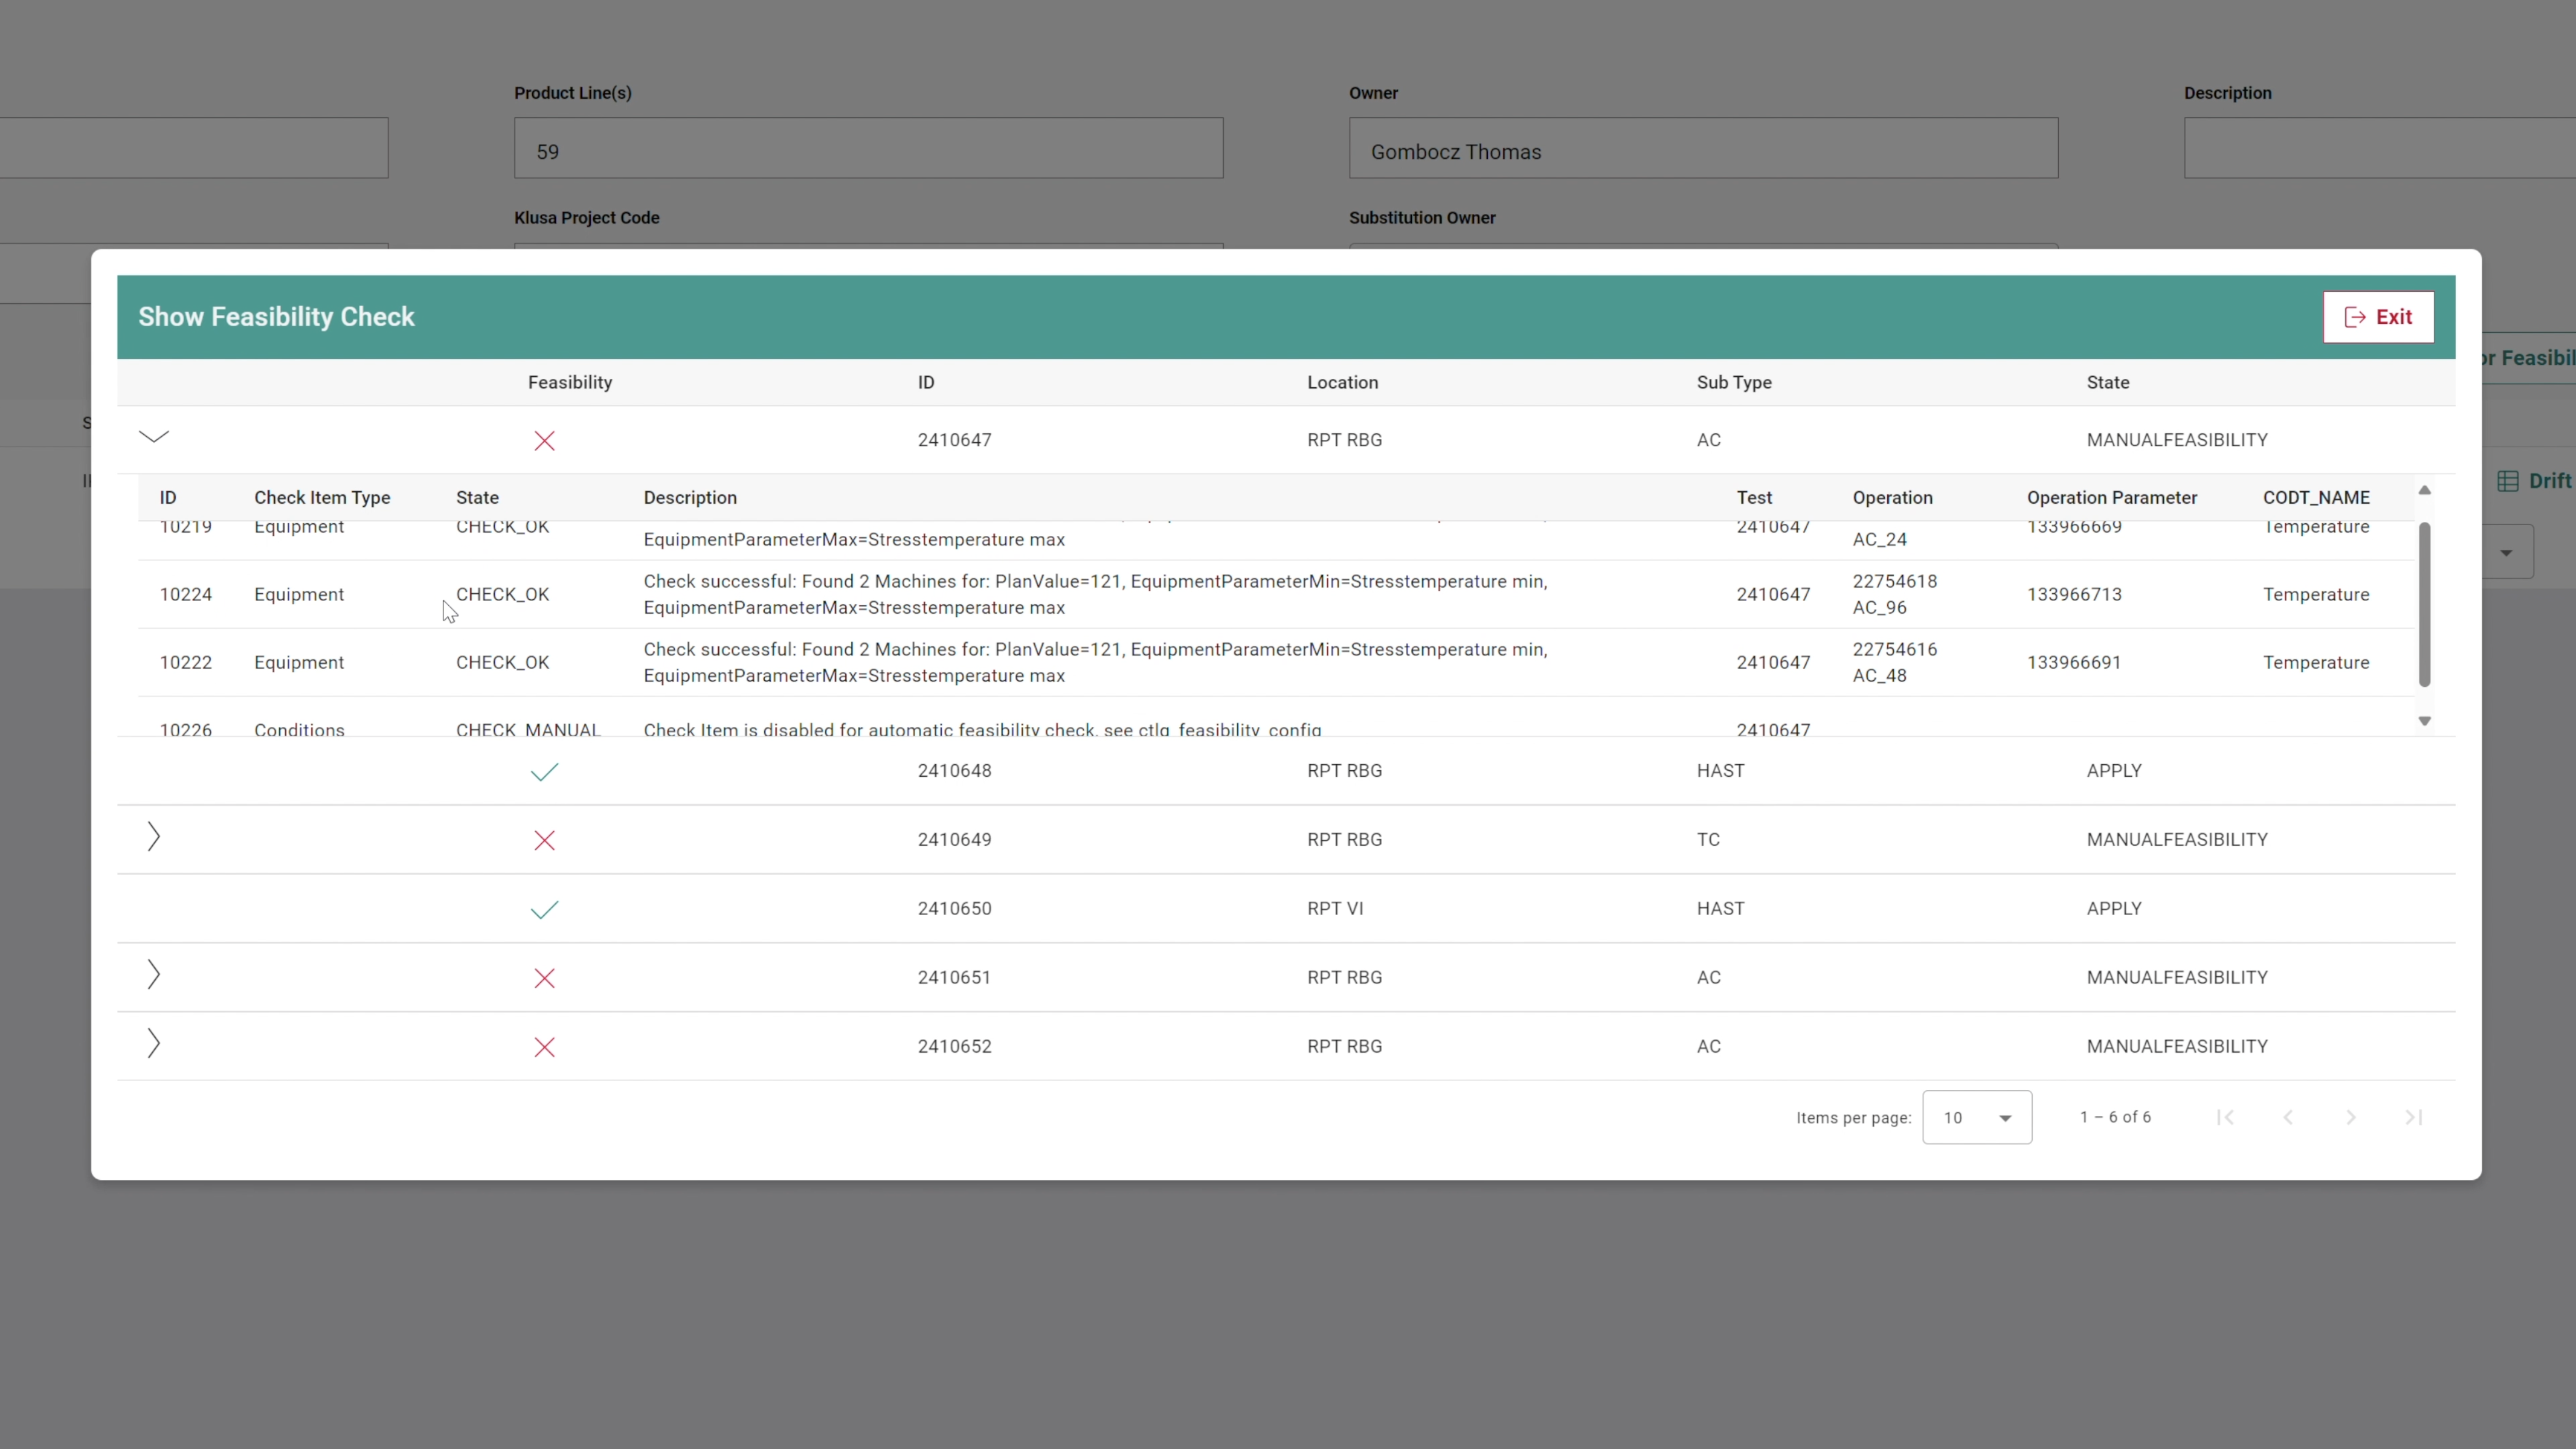
\includegraphics[width=0.85\paperwidth]{bilder/frontend/result-details.png}} 
    \caption{Modal-Page ''Submit Feasibility'' – Detaillierte Ergebnisse des Feasibility Checks} 
    \label{fig:result-details} 
\end{figure}

Das Popup-Fenster zeigt eine Tabelle mit allen Tests, ihren Informationen und den zugehörigen Ergebnissen. Der Benutzer kann einzelne Testzeilen aufklappen, um weitere Details zu erhalten. Links in der Tabelle sind Icons zu sehen, die anzeigen, welche Zeilen aufgeklappt werden können und welche aktuell geöffnet sind – dabei kann immer nur eine Zeile gleichzeitig ausgeklappt werden. 

In der aufgeklappten Ansicht werden in tabellarischen Form die gespeicherten \texttt{feasibility\_check\_item\_results}, des zugehörigen Tests angezeigt. Bei Tests die nur Überprüfungen mit dem Status-Ergebnis \texttt{''CHECK\_OFF''} aufweisen, liefern keine zusätzlichen Details, da in diesem Fall keine Feasibility-Resultate abgespeichert wurden. 

In der Spalte ''Check Item Type'' wird angegeben, ob es sich um einen Condition- oder Equipment Check handelt. In der Spalte ''State'' erscheint der Status, wie er in der Backend-Logik als Enum definiert ist. Zudem wird eine Beschreibung angezeigt, die dem Benutzer detaillierte Informationen zum jeweiligen Check liefert. Falls vorhanden, werden auch der zugehörige Operationstyp und die Parameter-ID dargestellt.

Diese Informationen sollen dem Benutzer helfen, die Ergebnisse nachvollziehen zu können. Außerdem ermöglichen sie es, bei unerwünschten Resultaten entsprechend zu reagieren. Entweder können die geplanten Tests und deren Parameter(-Werte) angepasst werden, oder weitere vom Feasibility Check abhängige Konditionen, wie etwa die Konfigurationstabelle können verändert werden.



